\chapter{Auswertung}
\label{ch:auswertung}

Die Metriken des Kriterienkatalogs werden in Abschnitt \ref{sec:zielgewichtung} gewichtet. Die Bewertung der Kriterien wird folgend im Detail vorgenommen und in Abschnitt \ref{sec:bewertung} zusammengefasst.

\section{Leistungsfähigkeit}
Die einzelnen Bestandteile der Messung der Leistungsfähigkeit werden ausgewertet. Dabei werden die Werte in Tabellen und Graphen dargestellt. Zur Zusammenfassung der Ergebnisse wird die Leistung der Kandidaten gegenüber Docker gewichtet und in Prozent angegeben. Docker entspricht 100\%. Die Konfidenzintervalle werden mit einem Signifikanzniveau von 95\% berechnet. Die Ergebnisse werden auf statistisch signifikante Unterschiede zwischen Docker und den jeweiligen Kandidaten untersucht. Die Werte in den Tabellen werden auf signifikante Stellen gerundet. Für Fälle ohne Messergebnisse ist ein "`-"' angegeben. Abschließend werden die Ergebnisse mithilfe der Gewichtung aus Abschnitt \ref{sec:zielgewichtung} für eine Bewertung verwendet.

\subsection{Webserverleistung}
Mithilfe des Programms ApacheBench wird die Leistung verschiedener Web"-server in Anfragen pro Sekunde für die einzelnen Kandidaten gemessen. Die detaillierte Auswertung kann der Tabelle \ref{tbl:abdetailauswertung} im Anhang entnommen werden. In den folgenden Fällen ist kein statistisch signifikanter Unterschied festzustellen und der Kandidat wird mit 100\% gewertet: Kata FC mit default Limits und der Skalierung acht bei Go Httpd, Kata mit minimalen Limits und der Skalierung eins bei Python Tornado, Kata mit maximalen Limits und der Skalierung eins und zwei bei Python Tornado und Kata mit default Limits und der Skalierung 8 bei Tomcat. Die Fälle werden in der Tabelle \ref{tbl:abdetailauswertung} grau markiert.

Die Ergebnisse werden nach Image und Limits gruppiert und sind der Tabelle \ref{tbl:abergebniss} zu entnehmen. Für die Images und die Limits wird ein Schnitt gebildet. Zusätzlich wird der Durchschnitt über alle Ergebnisse nach Kandidat angegeben. Die Werte werden nach dem Skalierungsverhalten in den Abbildungen \ref{fig:ab_go}, \ref{fig:ab_httpd}, \ref{fig:ab_nginx}, \ref{fig:ab_python} und \ref{fig:ab_tomcat} visualisiert. Die Konfidenzintervalle sind in diesen Grafiken eingezeichnet.

Die Leistung von Kata liegt bei den Images Go Httpd und Tomcat vor Docker, bei allen anderen Images liegt Kata über 20\% hinter Docker. 
Kata FC ist bei Go Httpd mit Docker vergleichbar, bei allen anderen Images über 30\% langsamer.
gVisor ist bei allen Images langsamer als Docker. Bei Python Tornado erreicht gVisor 50\% der Leistung von Docker.
Nabla ist bei den beiden betrachteten Images Go Httpd und Python Tornado schneller als Docker.
Im Durchschnitt erreicht Nabla eine Leistung von ca. 117\%, Kata von 110\%, Kata FC von 61\%, und gVisor von 35\%.
Wenn nur die Images Go Httpd und Python Tornado betrachtet werden, für die bei allen Kandidaten Messdaten vorliegen, verändert sich das Ergebnis geringfügig: Im Durchschnitt erreicht Kata hier eine Leistung von ca. 120\%, Nabla von 117\%, Kata FC von 84\%, und gVisor von 40\%.

\begin{table}[h]
	\small 
	\myfloatalign
	\begin{tabularx}{\textwidth}{Xlrrrrr} \hline
		\spacedlowsmallcaps{Image} & \spacedlowsmallcaps{Limit} & \spacedlowsmallcaps{Docker} & \spacedlowsmallcaps{Kata} & \spacedlowsmallcaps{Kata FC} & \spacedlowsmallcaps{gVisor} & \spacedlowsmallcaps{Nabla} \\ \hline
		go-httpd                & default          & 100,00     & 135,07 & 83,38   & 38,29  & 114,59 \\
		go-httpd                & min              & 100,00     & 230,43 & 137,32  & 23,68  & 156,90  \\
		go-httpd                & max              & 100,00     & 121,23 & 81,59   & 37,95  & 111,95 \\ \hline
		\multicolumn{2}{l}{\textbf{Schnitt go-httpd}}       & 100,00     & 162,24 & 100,76  & 33,31  & 127,81 \\ \hline
		httpd                   & default          & 100,00     & 29,57  & 21,15   & -      & -      \\
		httpd                   & min              & 100,00     & 149,56 & 68,53   & -      & -      \\
		httpd                   & max              & 100,00     & 41,78  & 21,23   & -      & -      \\ \hline
		\multicolumn{2}{l}{\textbf{Schnitt httpd}}          & 100,00     & 73,64  & 36,97   & -      & -      \\ \hline
		nginx                   & default          & 100,00     & 56,92  & 39,20    & 38,09  & -      \\
		nginx                   & min              & 100,00     & 91,58  & 39,52   & 24,66  & -      \\
		nginx                   & max              & 100,00     & 51,15  & 38,76   & 37,80   & -      \\ \hline
		\multicolumn{2}{l}{\textbf{Schnitt nginx}}          & 100,00     & 66,55  & 39,16   & 33,52  & -      \\ \hline
		python-tornado          & default          & 100,00     & 82,06  & 66,75   & 54,43  & 107,34 \\
		python-tornado          & min              & 100,00     & 75,23  & 66,18   & 32,06  & 107,16 \\
		python-tornado          & max              & 100,00     & 76,59  & 66,34   & 54,26  & 105,78 \\ \hline
		\multicolumn{2}{l}{\textbf{Schnitt python-tornado}} & 100,00     & 77,96  & 66,42   & 46,92  & 106,76 \\ \hline
		tomcat                  & default          & 100,00     & 81,14  & -       & 29,83  & -      \\
		tomcat                  & min              & 100,00     & 319,68 & -       & 18,15  & -      \\
		tomcat                  & max              & 100,00     & 106,09 & -       & 30,02  & -      \\ \hline
		\multicolumn{2}{l}{\textbf{Schnitt tomcat}}         & 100,00     & 168,97 & -       & 26,00     & -      \\ \hline
		&                  &        &        &         &        &        \\ \hline
		\textbf{Schnitt}                 &                  & 100,00     & 109,87 & 60,83   & 34,94  & 117,29 \\ 
		\hline
	\end{tabularx}
	\caption[Ergebnisse des ApacheBench Benchmarks]{Ergebnisse des ApacheBench Benchmarks}
	\footnotesize alle Angaben in Prozent, Werte größer 100 sind besser
	\label{tbl:abergebniss}
\end{table}

Werden die Ergebnisse nach den Ressourcenlimits gruppiert, vgl. Tabelle \ref{tbl:abnachlimits}, wird ersichtlich, dass Kata, Kata FC und Nabla bei einem minimalen Limit bessere Leistungen erzielten als bei einem Maximalen. Gerade bei der Ausführung von nur einem Container, liegen Kata und Nabla weit vor Docker: In diesem Fall erreicht beispielsweise Kata 683\%, Kata FC 374\% und Nabla 280\% der Leistung von Docker bei  Go Httpd, vgl. Tabelle \ref{tbl:abdetailauswertung}.

Die Kurven der verschiedenen Ressourcenlimits von Kata FC und Nabla liegen fast aufeinander, vgl. Abbildung \ref{fig:ab_go} und \ref{fig:ab_python}, daher ist anzunehmen, dass die Ressourcenlimits keine Auswirkungen auf die Leistungsfähigkeit haben.
Bei den meisten Images bleibt die Leistung von gVisor und Kata FC mit steigender Skalierung konstant. Docker hat bei zwei Containern mit den Images Httpd, Nginx und Tomcat ein lokales Maximum, bei drei Containern sinkt die Leistung und erst bei höheren Skalierungen wird das lokale Maximum wieder erreicht oder übertroffen. Kata zeigt ein ähnliches Verhalten mit dem default Limit bei fünf Containern mit den Images Httpd, Nginx und Tomcat.
Bei jedem Image gibt es mindestens eine Runtime, die ihr Maximum noch nicht erreicht hat oder sich einem konstanten Wert annähert. So steigen Docker, Kata und Nabla über die betrachteten Skalierungsstufen. 

\begin{table}[h]
	\small 
	\myfloatalign
	\begin{tabularx}{\textwidth}{Xlrrrrr} \hline
		& \spacedlowsmallcaps{Limit} & \spacedlowsmallcaps{Docker} & \spacedlowsmallcaps{Kata} & \spacedlowsmallcaps{Kata FC} & \spacedlowsmallcaps{gVisor} & \spacedlowsmallcaps{Nabla} \\ \hline
		Schnitt & default & 100,00    & 76,95 & 52,62   & 40,16  & 110,97 \\
		Schnitt & min     & 100,00     & 173,30 & 77,89   & 24,64  & 132,03 \\
		Schnitt & max     & 100,00     & 79,37 & 51,98   & 40,01  & 108,87 \\
		\hline
	\end{tabularx}
	\caption[Ergebnisse ApacheBench nach Limits]{Ergebnisse des ApacheBench Benchmarks nach den Ressourcenlimits}
	\footnotesize alle Angaben in Prozent, Werte größer 100 sind besser
	\label{tbl:abnachlimits}
\end{table}

In der Literatur wird ein ApachBench Benchmark mit Nginx für Docker, Kata und gVisor durchgeführt. Dabei hat Kata eine vergleichbare Leistung wie Docker und gVisor eine Leistung von etwa zwei Prozent \cite[vgl.][23]{XuWang.2018}. Die Rangfolge der Kandidaten stimmt mit der Messung der vorliegenden Arbeit überein. Die Verhältnisse entsprechen aber keiner Messung mit dem Nginx Image. In der Quelle wird der Messaufbau nicht genau beschrieben, daher ist es schwer, einen Vergleich vorzunehmen.


\begin{figure}[h]
	\myfloatalign
	\subfloat[Anfragen pro Sekunde nach Skalierungsstufen für Go Httpd]
	{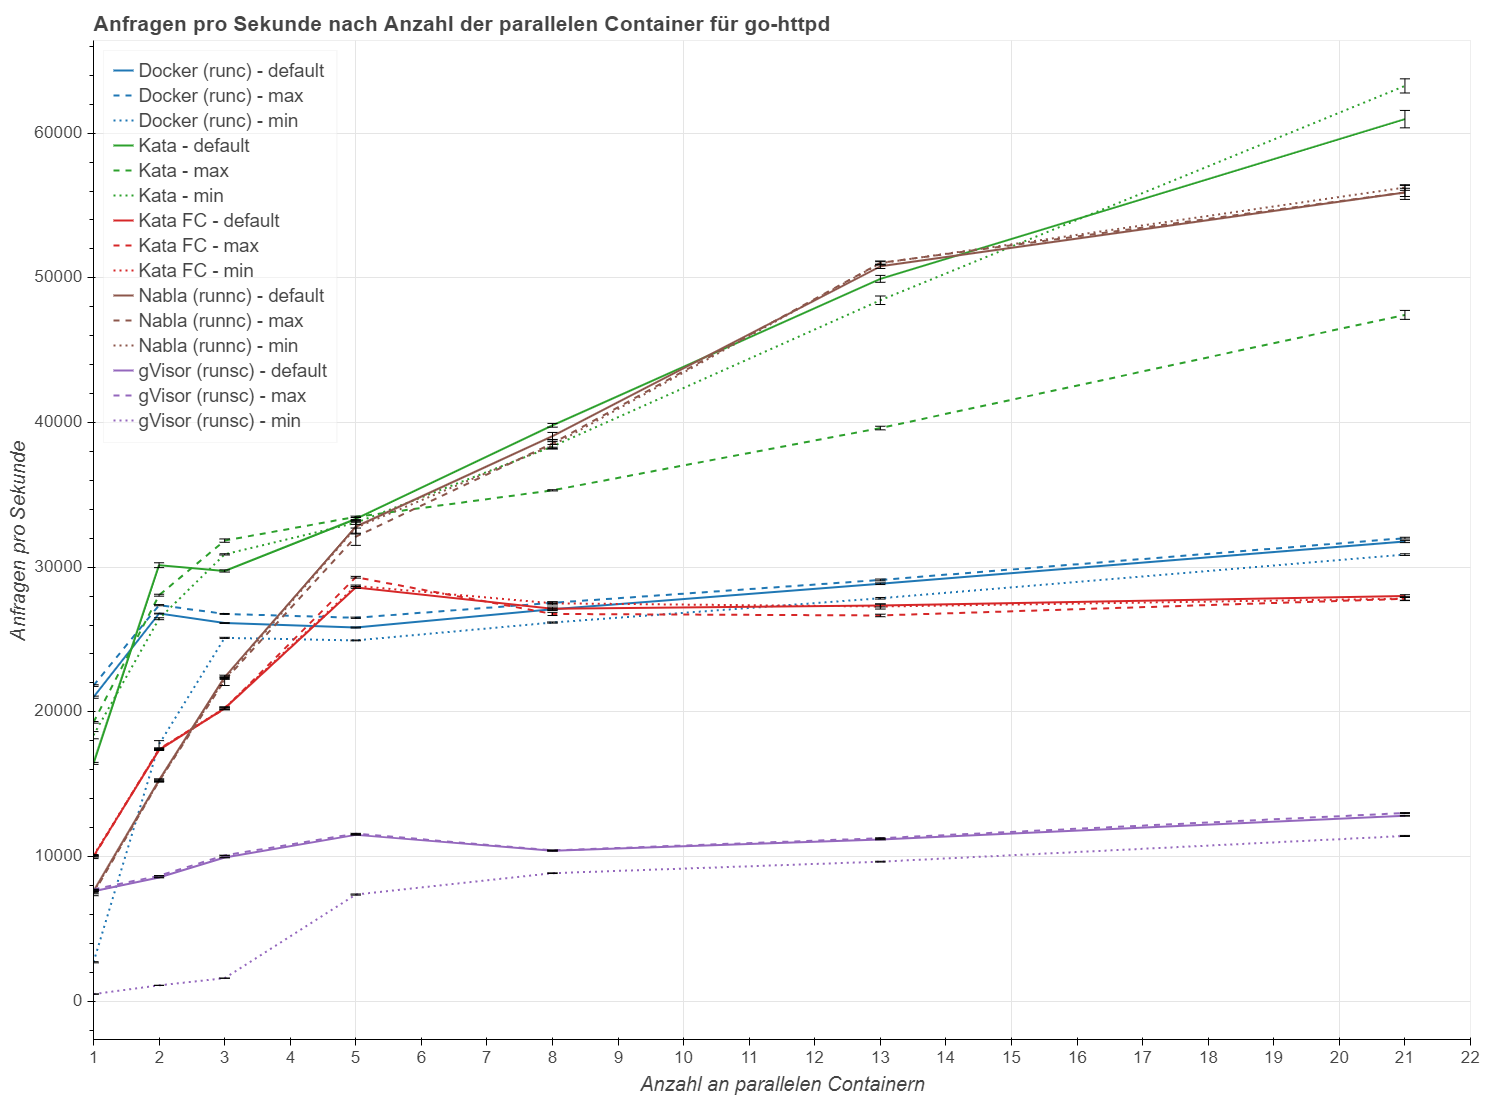
\includegraphics[width=0.98\linewidth]{gfx/auswertung/ab_go.png} 
		\label{fig:ab_go}}
		\caption{Anfragen pro Sekunde nach Skalierungsstufen}
	\end{figure}

	\begin{figure}[]
	\captionsetup{list=no}
	\ContinuedFloat 
	\centering 
	\subfloat[Anfragen pro Sekunde nach Skalierungsstufen für Httpd]
	{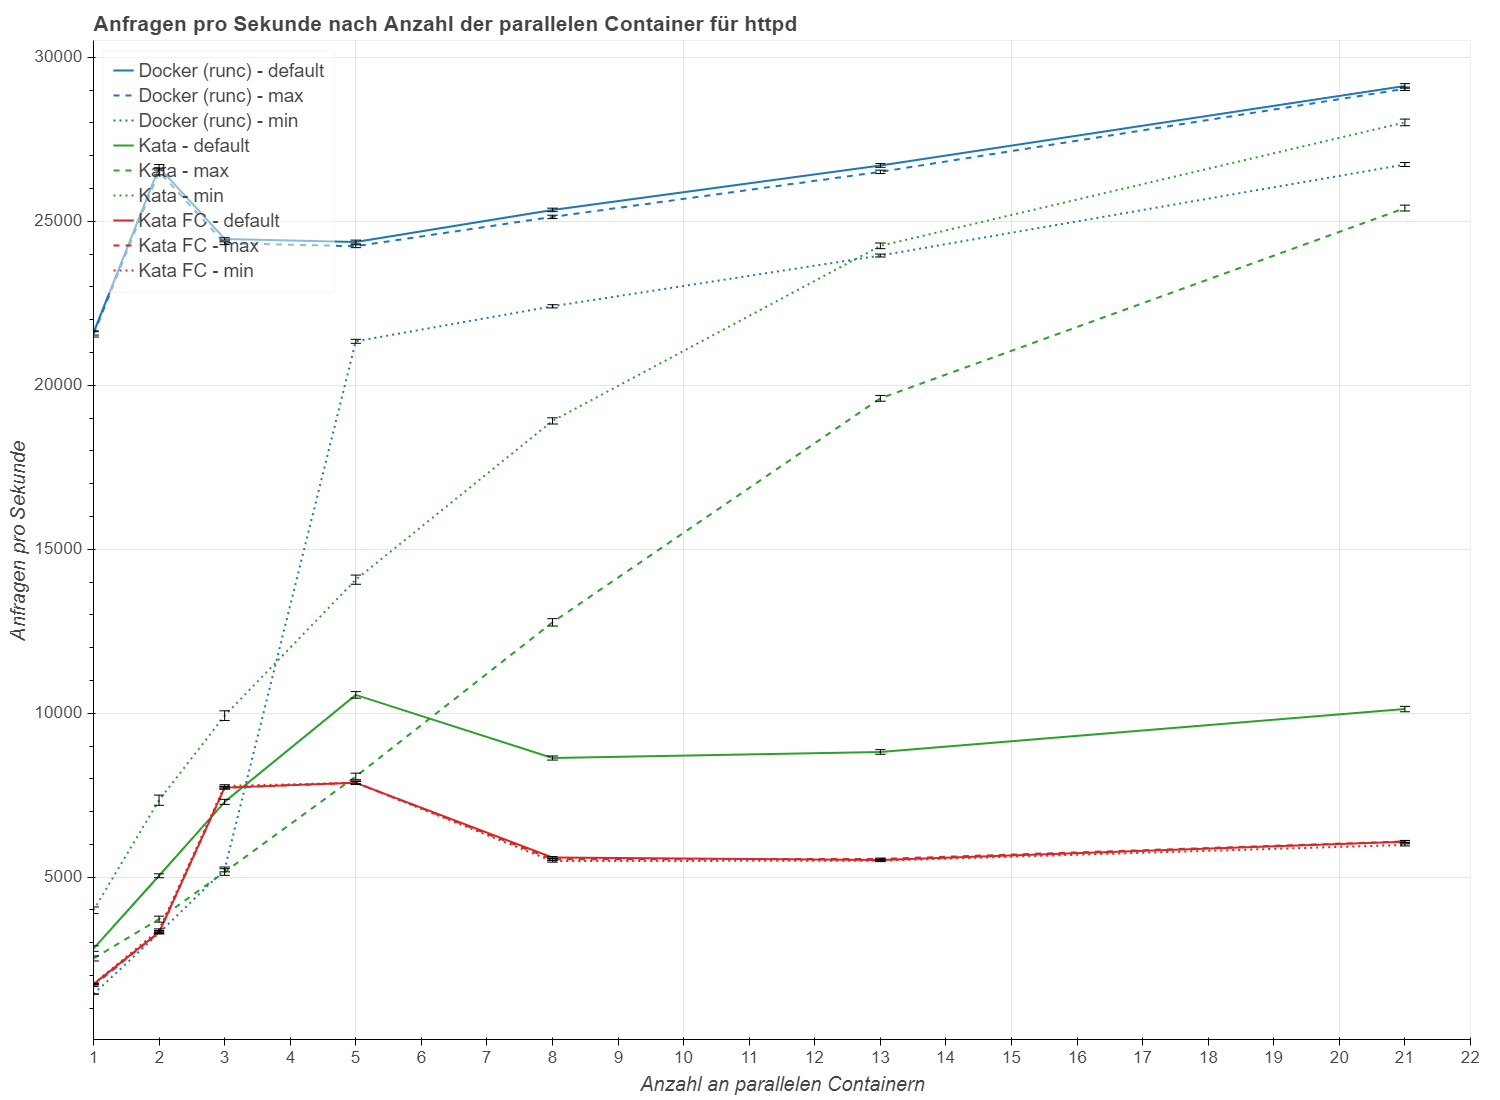
\includegraphics[width=0.98\linewidth]{gfx/auswertung/ab_httpd.png}
		\label{fig:ab_httpd}} \\
	\subfloat[Anfragen pro Sekunde nach Skalierungsstufen für Nginx]
	{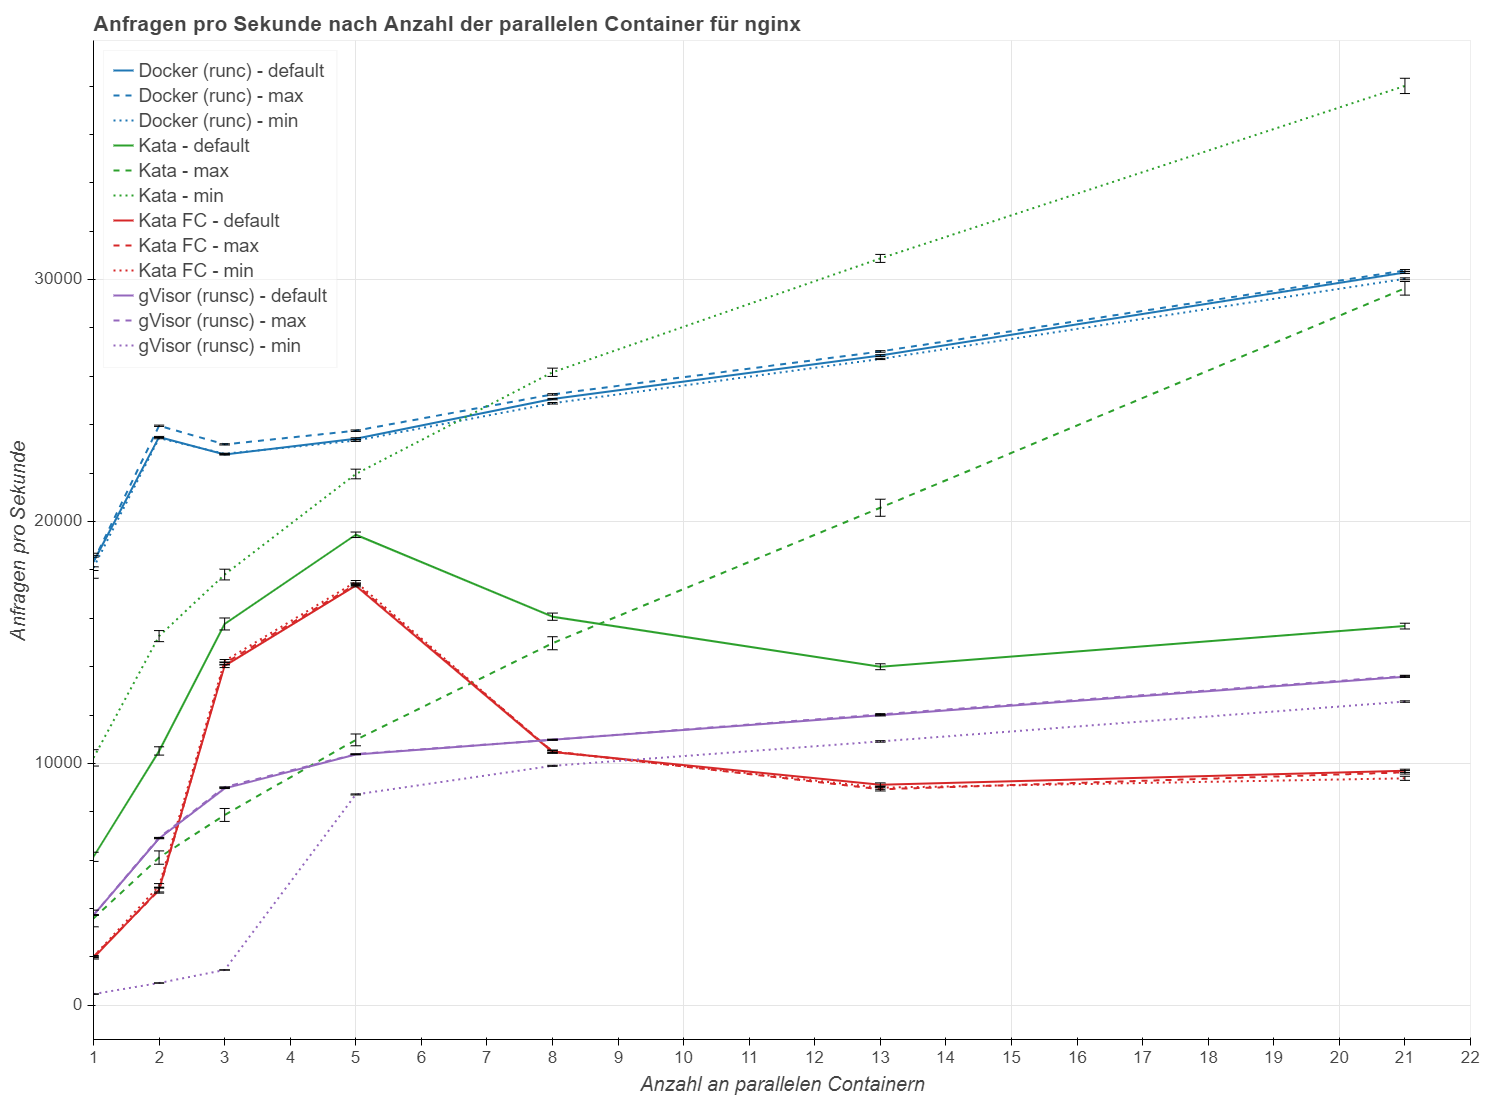
\includegraphics[width=0.98\linewidth]{gfx/auswertung/ab_nginx.png} 
		\label{fig:ab_nginx}}
	\caption{Anfragen pro Sekunde nach Skalierungsstufen}
\end{figure}

\begin{figure}[]
	\captionsetup{list=no}
	\ContinuedFloat 
	\centering 
	\subfloat[Anfragen pro Sekunde nach Skalierungsstufen für Python Tornado]
	{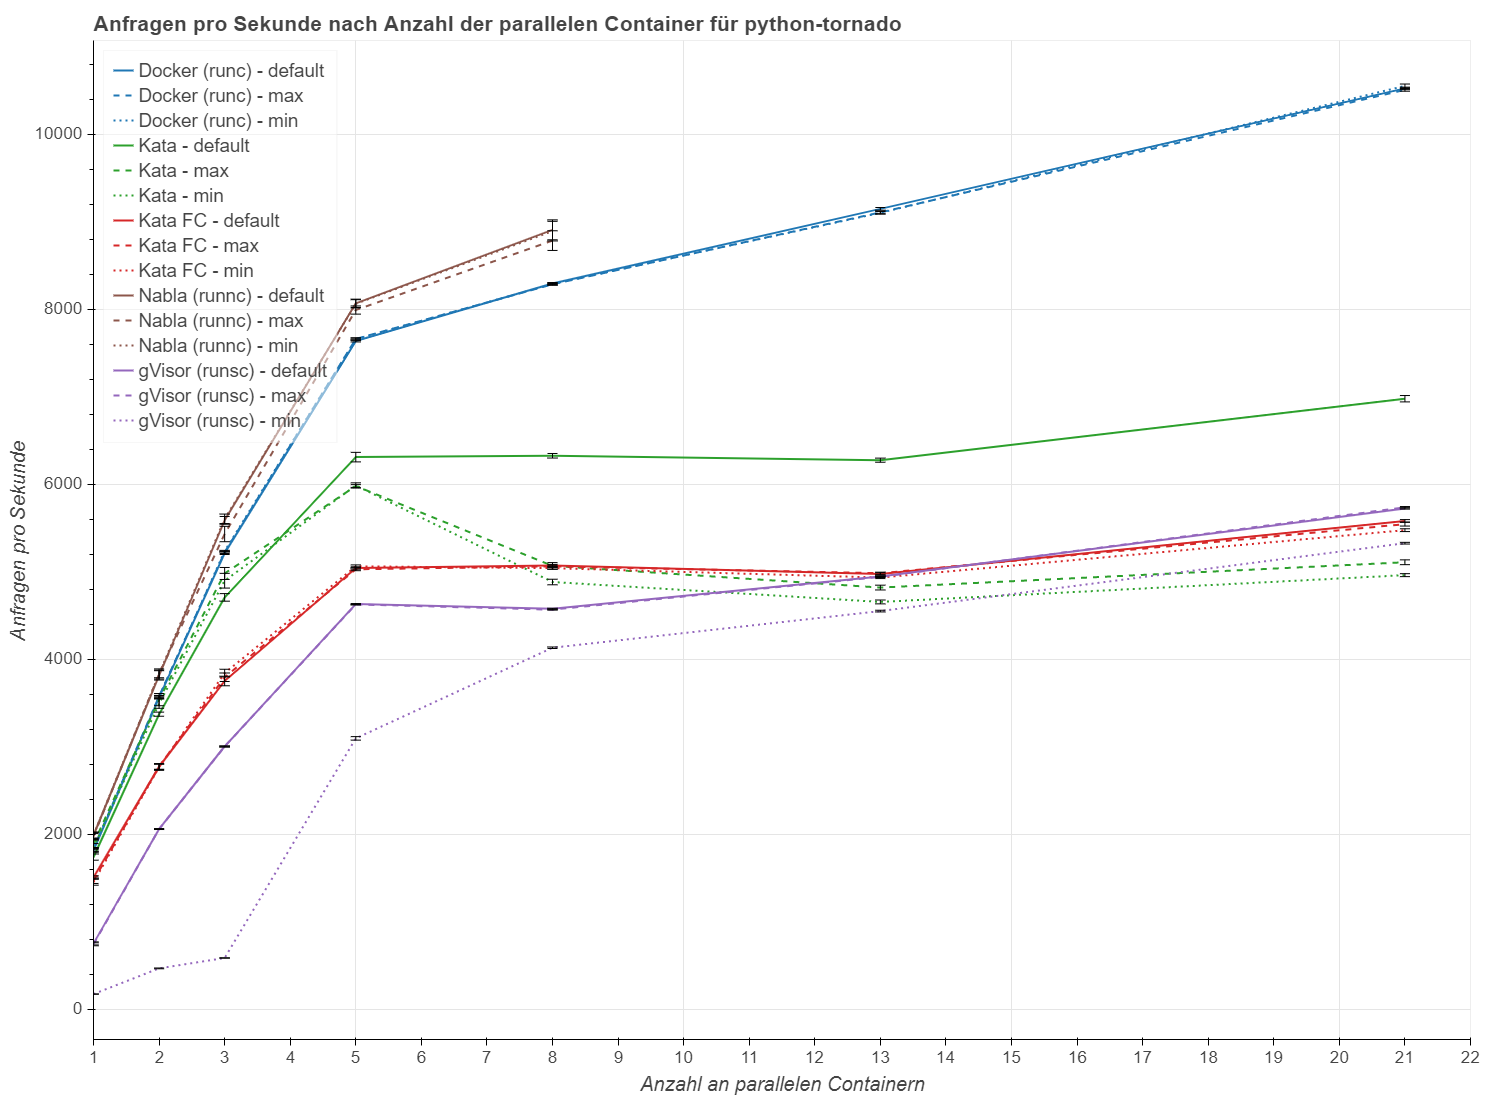
\includegraphics[width=0.98\linewidth]{gfx/auswertung/ab_python.png}
		\label{fig:ab_python}} \\
	\subfloat[Anfragen pro Sekunde nach Skalierungsstufen für Tomcat]
	{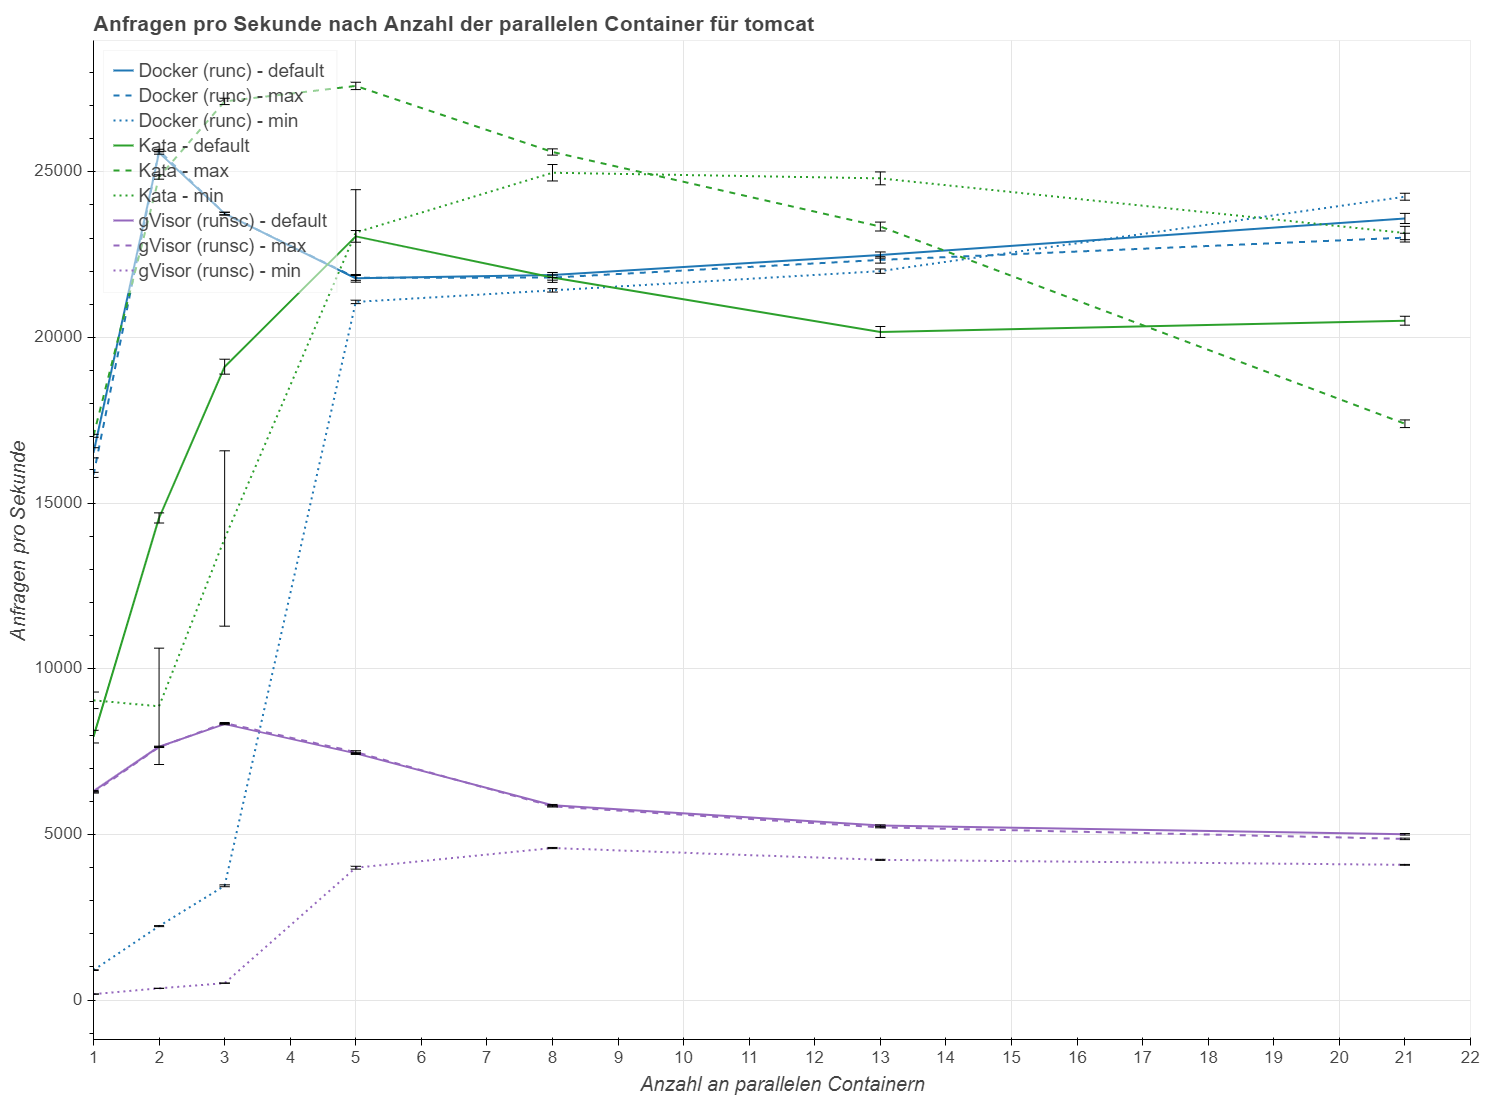
\includegraphics[width=0.98\linewidth]{gfx/auswertung/ab_tomcat.png} 
		\label{fig:ab_tomcat}}
	\caption{Anfragen pro Sekunde nach Skalierungsstufen}
\end{figure}


\subsection{Arbeitsspeicherverbrauch}
Während des ApacheBench Benchmarks wird der verwendete Arbeitsspeicher des Linux Systems gemessen. Die detaillierten Ergebnisse sind der Tabelle \ref{tbl:ramdetailauswertung} im Anhang zu entnehmen. Die Werte sind nach dem Skalierungsverhalten in den Graphen \ref{fig:ram_go}, \ref{fig:ram_httpd}, \ref{fig:ram_nginx}, \ref{fig:ram_python} und \ref{fig:ram_tomcat} visualisiert. Die Konfidenzintervalle sind in diesen Grafiken eingezeichnet.

Wenn kein statistisch signifikanter Unterschied zu Docker festzustellen ist, wird der Kandidat mit 100\% gewertet und in der Tabelle \ref{tbl:ramdetailauswertung} grau markiert.
Die Ergebnisse sind nach Image und Limits gruppiert und der Tabelle \ref{tbl:ramergebnis} zu entnehmen. Für die Images und die Limits wird der Schnitt gebildet. Weiter ist der Durchschnitt über alle Ergebnisse nach Kandidat angegeben. 

\begin{table}[h]
	\myfloatalign
	\small 
	\begin{tabularx}{\textwidth}{Xlrrrrr} \hline
		\spacedlowsmallcaps{Image} & \spacedlowsmallcaps{Limit} & \spacedlowsmallcaps{Docker} & \spacedlowsmallcaps{Kata} & \spacedlowsmallcaps{Kata FC} & \spacedlowsmallcaps{gVisor} & \spacedlowsmallcaps{Nabla} \\ \hline
		go-httpd & default & 100,00 & 157,12 & 87,88 & 304,29 & 93,70 \\
		go-httpd & min & 100,00 & 231,18 & 106,37 & 133,48 & 114,44 \\
		go-httpd & max & 100,00 & 407,58 & 105,11 & 164,06 & 119,50 \\ \hline
		\multicolumn{2}{l}{\textbf{Schnitt go-httpd}} & 100,00 & 265,29 & 99,75 & 200,61 & 109,20 \\ \hline
		httpd & default & 100,00 & 178,78 & 82,36 & - & - \\
		httpd & min & 100,00 & 219,09 & 83,64 & - & - \\
		httpd & max & 100,00 & 363,18 & 185,08 & - & - \\ \hline
		\multicolumn{2}{l}{\textbf{Schnitt httpd}} & 100,00 & 253,68 & 117,03 & - & - \\ \hline
		nginx & default & 100,00 & 145,12 & 96,61 & 123,78 & - \\
		nginx & min & 100,00 & 159,48 & 100,85 & 112,20 & - \\
		nginx & max & 100,00 & 238,15 & 112,98 & 112,97 & - \\ \hline
		\multicolumn{2}{l}{\textbf{Schnitt nginx}} & 100,00 & 180,92 & 103,48 & 116,32 & - \\ \hline
		python-tornado & default & 100,00 & 114,75 & 90,27 & 121,87 & 37,82 \\
		python-tornado & min & 100,00 & 139,81 & 93,49 & 104,21 & 41,02 \\
		python-tornado & max & 100,00 & 139,81 & 99,51 & 109,06 & 40,90\\ \hline
		\multicolumn{2}{l}{\textbf{Schnitt python-tornado}} & 100,00 & 131,46 & 94,42 & 111,71 & 39,91 \\ \hline
		tomcat & default & 100,00 & 126,76 & - & 59,45 & - \\
		tomcat & min & 100,00 & 160,05 & - & 28,04 & - \\
		tomcat & max & 100,00 & 175,58 & - & 34,69 & - \\ \hline
		\multicolumn{2}{l}{\textbf{Schnitt tomcat}} & 100,00 & 154,13 & - & 40,73 & - \\ \hline
		\textbf{Schnitt} & & 100,00 & 197,10 & 103,67 & 117,34 & 74,56 \\
		\hline
	\end{tabularx}
	\caption[Ergebnisse des Arbeitsspeicherverbrauchs Benchmarks]{Ergebnisse des Arbeitsspeicherverbrauchs Benchmarks}
	\footnotesize alle Angaben in Prozent, Werte kleiner 100 sind besser
	\label{tbl:ramergebnis}
\end{table}

Da mit der Messmethode das gesamte Linux System betrachtet wird, sind die Ergebnisse nicht exakt, daraus lassen sich aber Tendenzen ableiten.
Der Arbeitsspeicherverbrauch liegt bei Kata deutlich über Docker. In machen Fällen ist er drei oder viermal so hoch. Im Durchschnitt ist er doppelt so hoch wie der von Docker. Kata FC benötigt meist den gleichen Speicherplatz wie Docker. Nur im Fall von Nginx mit maximalen Limits belegt Kata FC 185\% des Speichers im Vergleich zu Docker. Der Verbrauch von gVisor bei den Images Nginx und Python Tornado liegt über dem von Docker. Im Betrieb von Go Httpd ist der Verbrauch doppelt so hoch, bei Tomcat weniger als halb so hoch. Nabla verwendet bei Go Httpd etwa gleich viel Arbeitsspeicher wie Docker, bei Python Tornado 40\%.

Insgesamt ist der Verbrauch von Kata fast doppelt so hoch wie der von Docker, was auf die Verwendung von Betriebssystemvirtualisierung zurückzuführen ist. Bei Kata FC ist die Arbeitsspeichernutzung mit Docker vergleichbar. Daraus lässt sich schließen, dass Firecracker weniger Arbeitsspeicher benötigt als Clear Linux und \ac{QEMU}.
gVisor liegt je nach Anwendungsfall über oder unter dem Verbrauch von Docker. Zusammenfassend ergibt sich ein Overhead von etwa 20\% im Speicherverbrauch. Beachtenswert ist, dass Nabla im Fall von Python Tornado deutlich unter dem Verbrauch von Docker liegt. 
Wird der Arbeitsspeicherverbrauch mit der Skalierung in Zusammenhang gebracht, wird ersichtlich, dass der Verbrauch mit steigender Skalierung zunimmt. Dabei ist die Steigung bei Kata am steilsten. Auffällig ist, dass sich für viele Runtimes der Tiefpunkt nicht bei einem, sondern bei zwei Containern befindet.
Die Kurven für die jeweiligen Limits liegen bei allen Runtimes dicht beieinander. Kata bildet die Ausnahme, bei dieser Runtime ist ein deutlicher Unterschied zwischen dem default und maximalen Limit ersichtlich.

\begin{figure}[h]
	\myfloatalign
	\subfloat[Arbeitsspeicherverbrauch nach Skalierungsstufen für Go Httpd]
	{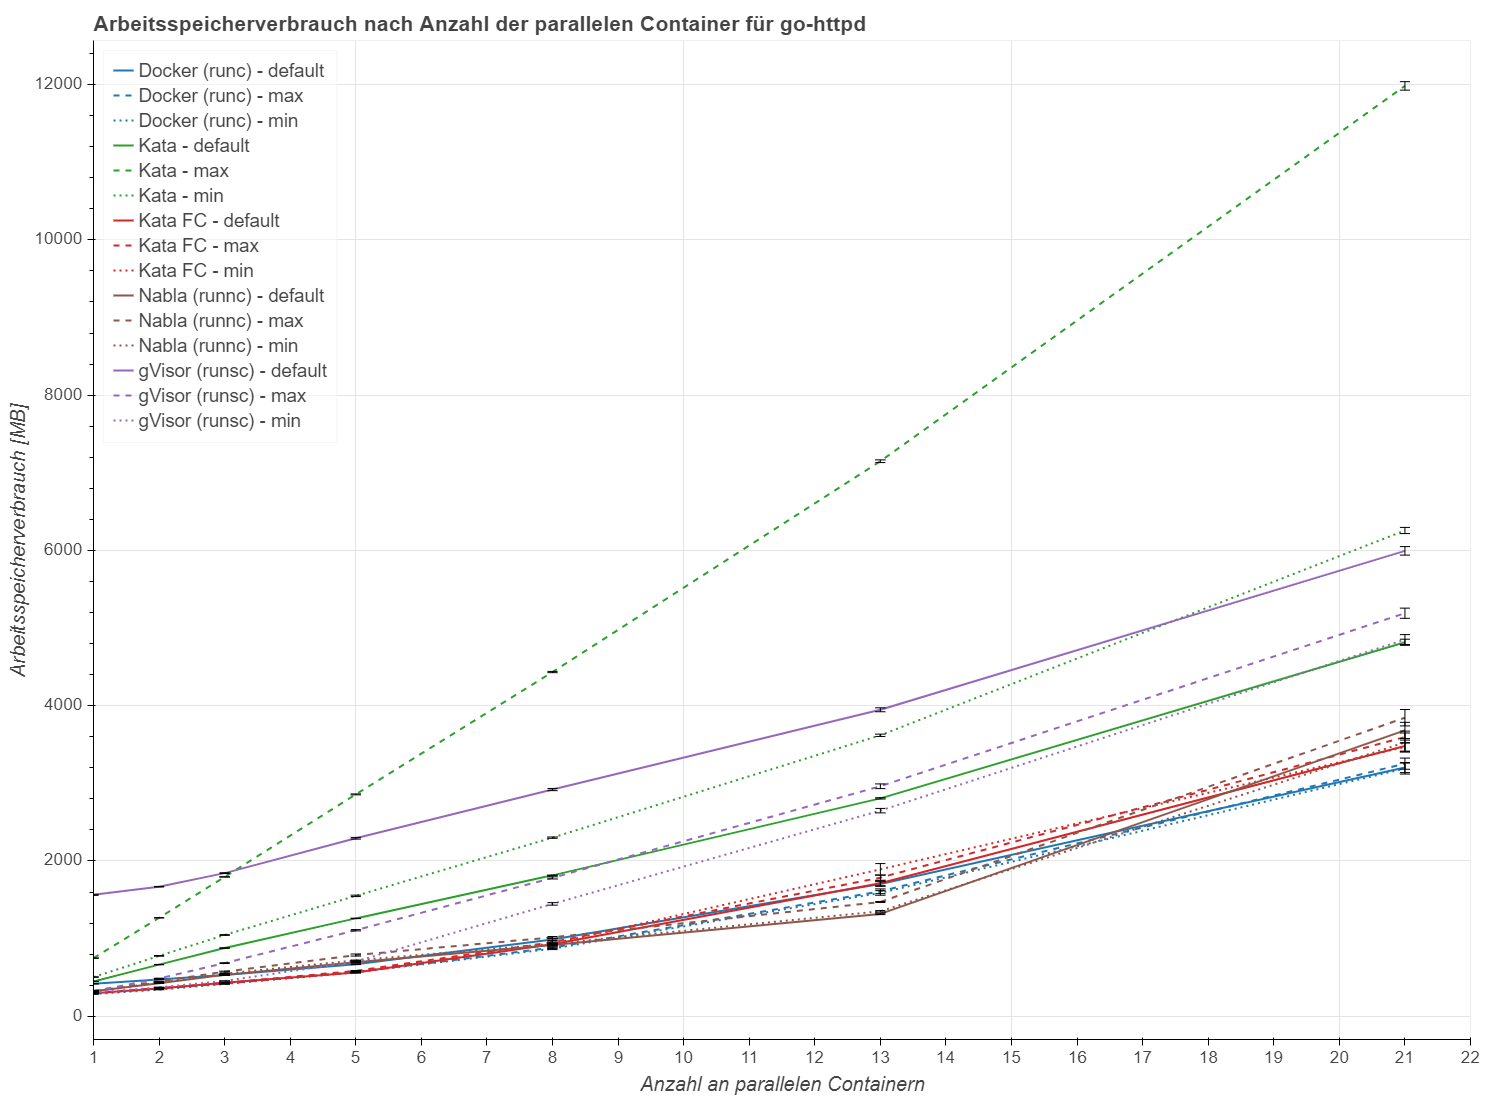
\includegraphics[width=0.98\linewidth]{gfx/auswertung/ram_go.png} 
		\label{fig:ram_go}} 
	\caption{Arbeitsspeicherverbrauch nach Skalierungsstufen}
\end{figure}

\begin{figure}[]
	\ContinuedFloat 
	\captionsetup{list=no}
	\centering 
	\subfloat[Arbeitsspeicherverbrauch nach Skalierungsstufen für Httpd]
	{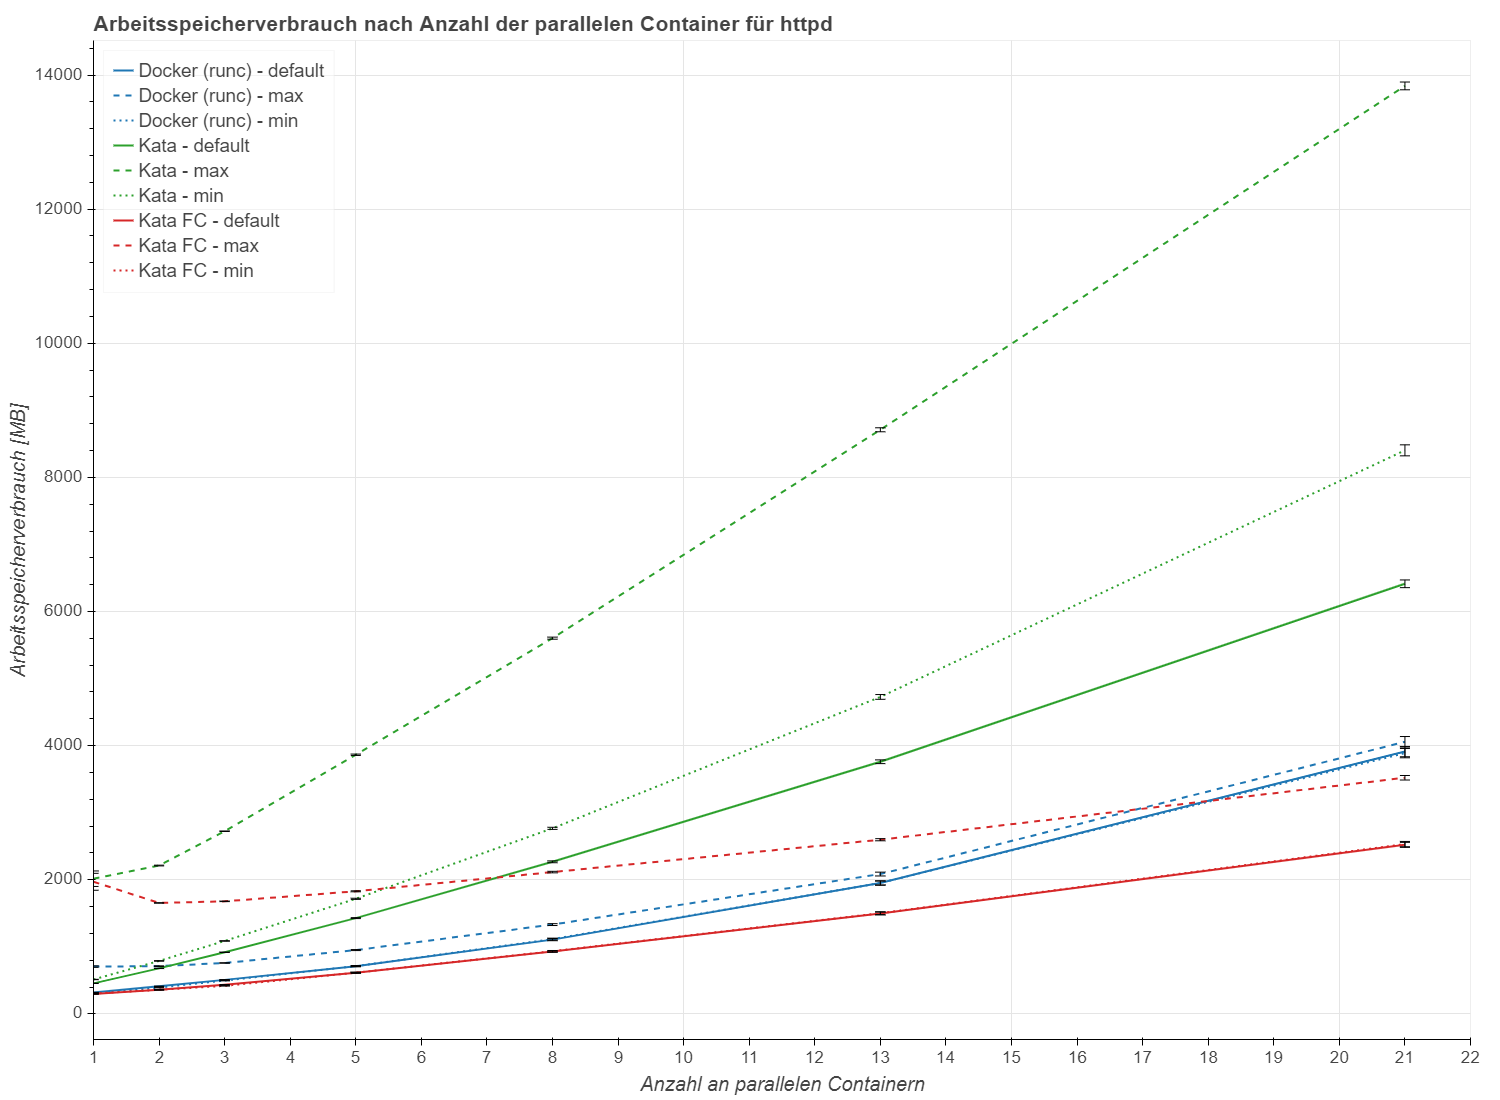
\includegraphics[width=0.98\linewidth]{gfx/auswertung/ram_httpd.png}
		\label{fig:ram_httpd}} \\
	\subfloat[Arbeitsspeicherverbrauch nach Skalierungsstufen für Nginx]
	{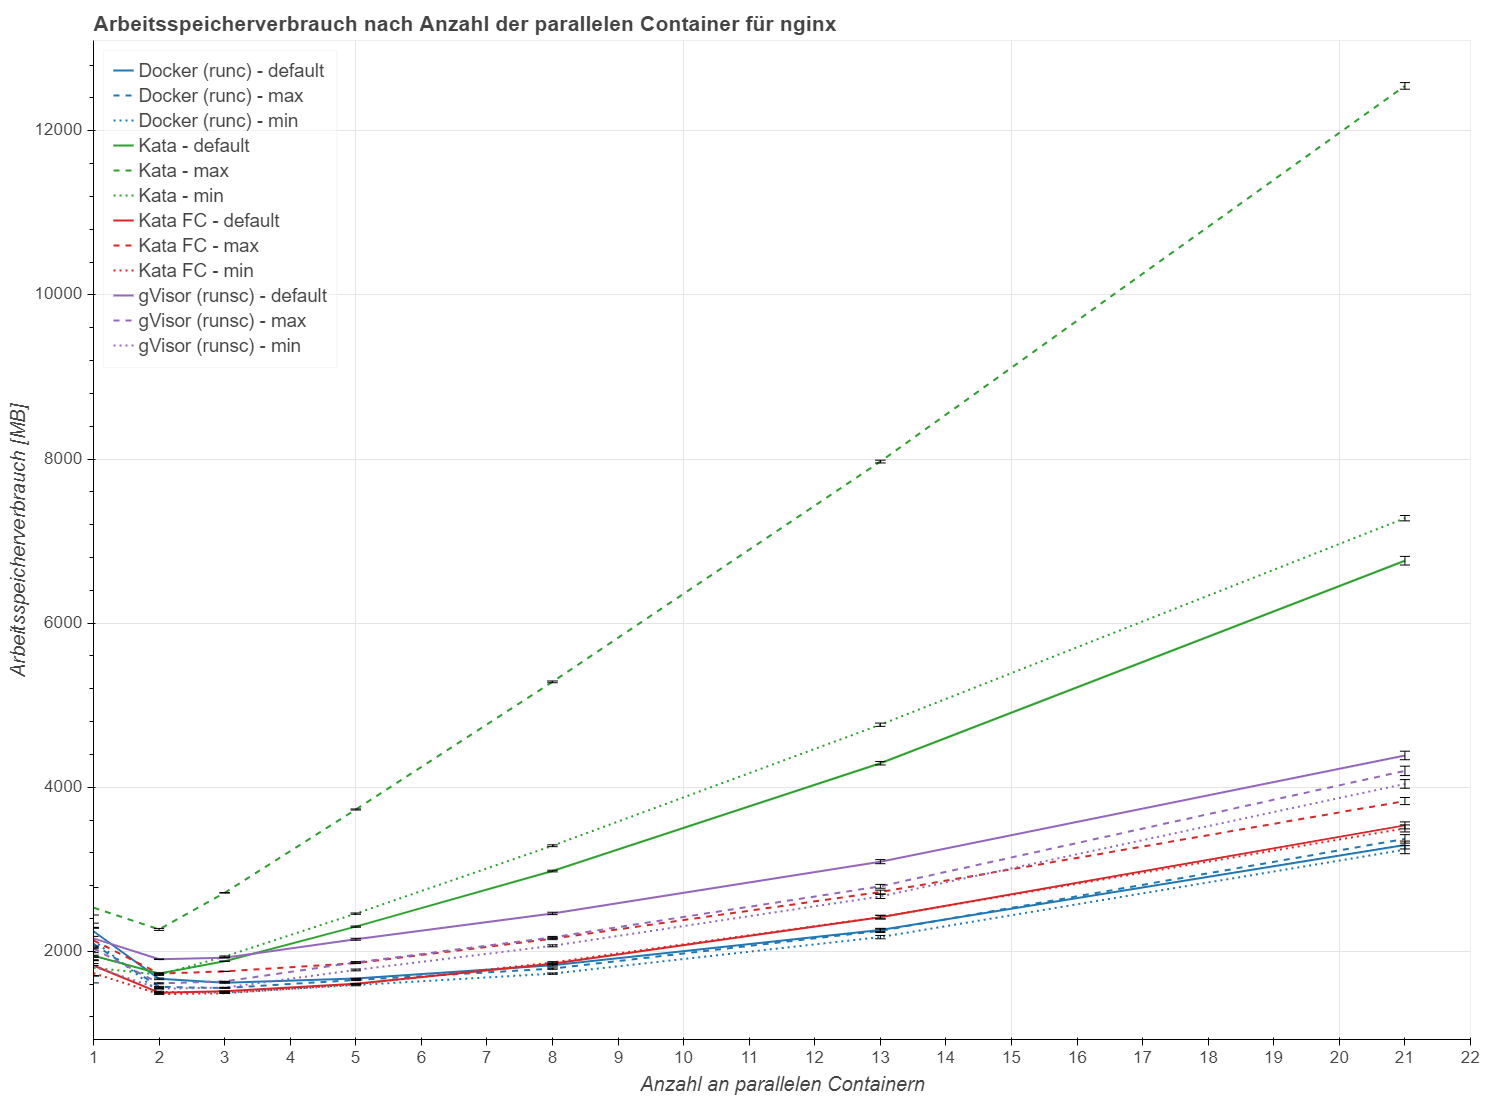
\includegraphics[width=0.98\linewidth]{gfx/auswertung/ram_nginx.png} 
		\label{fig:ram_nginx}} \\
	\caption{Arbeitsspeicherverbrauch nach Skalierungsstufen}
\end{figure}

\begin{figure}[]
	\ContinuedFloat 
	\centering 
	\captionsetup{list=no}
	\subfloat[Arbeitsspeicherverbrauch nach Skalierungsstufen für Python Tornado]
	{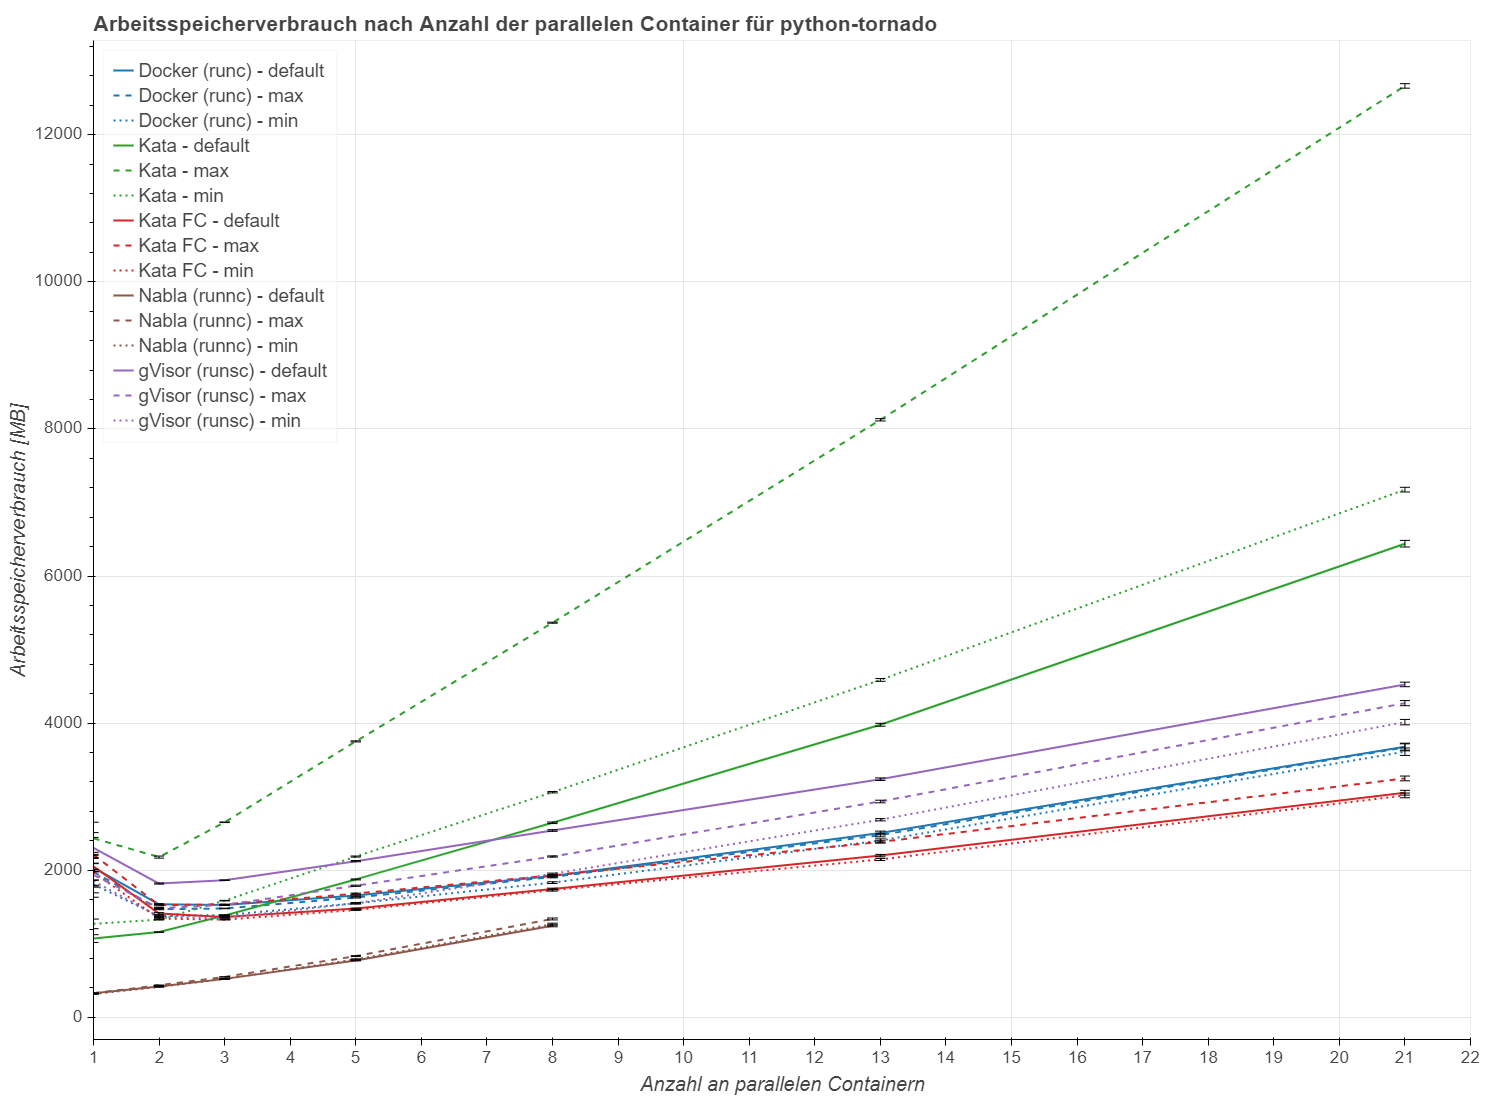
\includegraphics[width=0.98\linewidth]{gfx/auswertung/ram_python.png}
		\label{fig:ram_python}} \\
	\subfloat[Arbeitsspeicherverbrauch nach Skalierungsstufen für Tomcat]
	{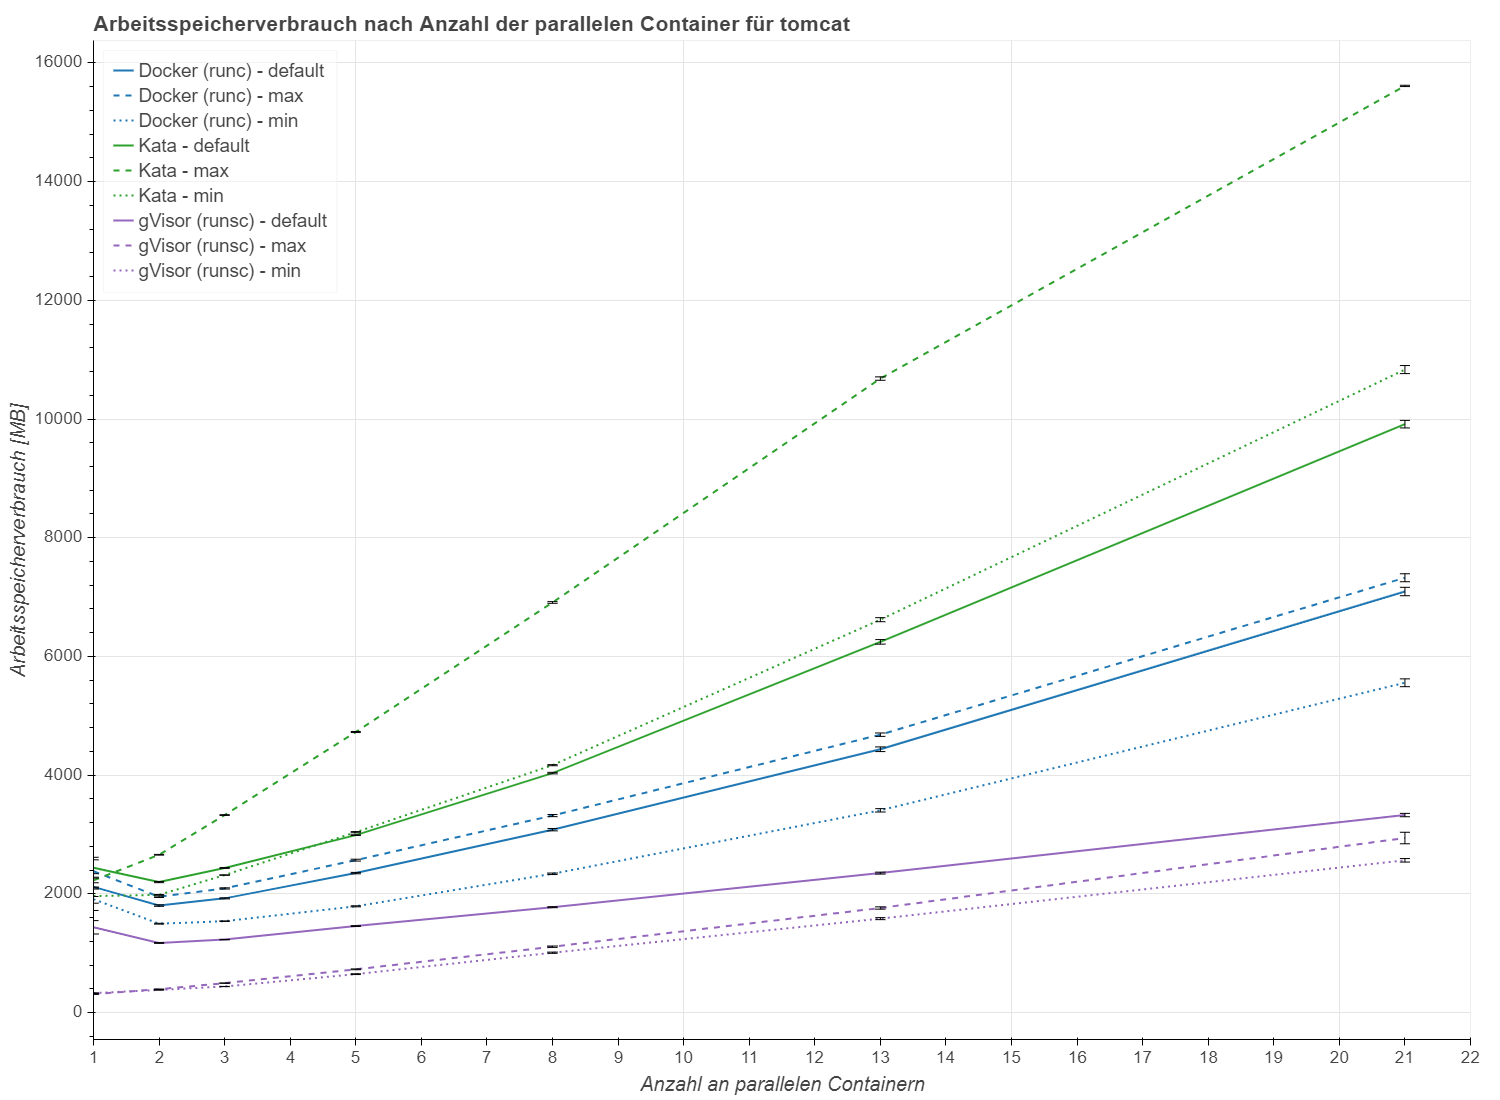
\includegraphics[width=0.98\linewidth]{gfx/auswertung/ram_tomcat.png} 
		\label{fig:ram_tomcat}}
	\caption{Arbeitsspeicherverbrauch nach Skalierungsstufen}
\end{figure}

\subsection{Dauer des Startens und Entfernens eines Containers}
Die Dauer der Containererzeugung und -entfernung wird mit dem Bash Programm time gemessen. Alle Fälle, in denen kein statistisch signifikanter Unterschied festzustellen ist, werden in den Tabellen \ref{tbl:timeuperfergebnis} und \ref{tbl:timermerfergebnis} im Anhang grau markiert und mit 100\% gewertet. Die Messergebnisse werden nach Image und Limits gruppiert und sind im Anhang den Tabellen \ref{tbl:timeuperfergebnis} für die Dauer des Startens und \ref{tbl:timermerfergebnis} für die Dauer des Entfernens zu entnehmen. Für die einzelnen Images und über alle Kandidaten wird der Durchschnitt gebildet. Für einen Überblick werden die Ergebnisse nach den Images gruppiert und sind Tabelle \ref{tbl:timeup} für die Dauer des Startens und Tabelle \ref{tbl:timerm} für die Dauer des Entfernens zu entnehmen.

\begin{table}[h]
	\myfloatalign
	\small 
	\begin{tabularx}{\textwidth}{Xrrrrr} \hline
		\spacedlowsmallcaps{Image} & \spacedlowsmallcaps{Docker} & \spacedlowsmallcaps{Kata} & \spacedlowsmallcaps{Kata FC} & \spacedlowsmallcaps{gVisor} & \spacedlowsmallcaps{Nabla} \\ \hline
		alpine        & 100,00 & 193,16 & 334,12  & 105,58 & -      \\
		busybox       & 100,00 & 192,29 & 326,89  & 103,38 & -      \\
		go-httpd      & 100,00 & 177,94 & 310,51  & 103,23 & 340,61 \\
		httpd         & 100,00 & 178,49 & 310,06  & 103,24 & -      \\
		mongo         & 100,00 & 179,48 & 306,90  & 106,42 & -      \\
		nginx         & 100,00 & 180,42 & 313,42  & 105,02 & -      \\
		node-express  & 100,00 & 182,36 & 315,07  & 104,60 & 345,77 \\
		postgres      & 100,00 & 179,24 & 308,22  & 107,04 & -      \\
		python-tornado& 100,00 & 179,96 & 312,69  & 103,65 & 135,31 \\
		redis-test    & 100,00 & 179,59 & 312,32  & 105,69 & 117,11 \\
		tomcat        & 100,00 & 180,08 & 312,87  & 106,27 & -      \\
		traefik       & 100,00 & 179,73 & 314,65  & 105,30 & -      \\
		ubuntu        & 100,00 & 196,58 & 334,35  & 105,41 & -      \\ \hline
		\textbf{Schnitt}   & 100,00 & 183,02 & 316,31  & 104,99 & 234,70 \\
		\hline
	\end{tabularx}
	\caption[Dauer des Startens eines Containers]{Dauer des Startens eines Containers nach den Images}
	\footnotesize alle Angaben in Prozent, Werte kleiner 100 sind besser
	\label{tbl:timeup}
\end{table}

Beim Starten eines Containers sind über alle Images hinweg klare Tendenzen sichtbar. Kata FC benötigt über die dreifache Zeit zum Starten verglichen mit Docker. GVisor ist nur wenig langsamer als Docker und bei Kata dauert der Start 180\% der Zeit von Docker. Bei Nabla liegen die Startzeiten bei den Images Go Httpd und Node Express mit ca. 340\% deutlich über den Werten und bei den Images Python Tornado und Redis mit 135\% und 117\% nur geringfügig über den Werten von Docker.

Bei der Untersuchung zur Dauer für das Entfernen eines Containers liegen die Werte näher beieinander. Kata ist mit 141\% und Kata FC mit 172\% langsamer als Docker. Die Zeiten von gVisor sind mit denen von Docker vergleichbar. Einzig Nabla ist beim Entfernen mit 62\% schneller als Docker.

Werden die Ergebnisse nach den Ressourcenlimits gruppiert, vgl. Tabelle \ref{tbl:timenachlimits}, wird deutlich, dass sich die Werte zwischen den Limits sowohl beim Starten, als auch beim Entfernen kaum unterscheiden. Einzig die Startzeiten bei Kata mit einem maximalen Ressourcenlimit sind deutlich über den Zeiten mit einem default Limit. 

\begin{table}[h]
	\small 
	\myfloatalign
	\begin{tabularx}{\textwidth}{Xrrrrr} \hline
		\spacedlowsmallcaps{Image} & \spacedlowsmallcaps{Docker} & \spacedlowsmallcaps{Kata} & \spacedlowsmallcaps{Kata FC} & \spacedlowsmallcaps{gVisor} & \spacedlowsmallcaps{Nabla} \\ \hline
		alpine        & 100,00 & 143,07 & 152,86  & 100,00 & -     \\
		busybox       & 100,00 & 145,56 & 159,10  & 100,00 & -     \\
		go-httpd      & 100,00 & 129,34 & 155,33  & 105,87 & 74,94 \\
		httpd         & 100,00 & 142,16 & 177,88  & 109,32 & -     \\
		mongo         & 100,00 & 148,24 & 198,84  & 110,67 & -     \\
		nginx         & 100,00 & 136,91 & 172,27  & 109,85 & -     \\
		node-express  & 100,00 & 134,91 & 171,84  & 107,98 & 72,03 \\
		postgres      & 100,00 & 142,36 & 214,06  & 106,54 & -     \\
		python-tornado& 100,00 & 148,22 & 154,91  & 76,26  & 48,43 \\
		redis-test    & 100,00 & 135,66 & 162,57  & 111,12 & 53,14 \\
		tomcat        & 100,00 & 135,04 & 173,71  & 107,00 & -     \\
		traefik       & 100,00 & 142,17 & 184,19  & 111,32 & -     \\
		ubuntu        & 100,00 & 143,48 & 154,68  & 108,34 & -     \\ \hline
		\textbf{Schnitt}                & 100,00 & 140,55 & 171,71  & 104,94 & 62,14\\
		\hline
	\end{tabularx}
	\caption[Dauer des Entfernens eines Containers]{Dauer des Entfernens eines Containers nach den Images}
	\footnotesize alle Angaben in Prozent, Werte kleiner 100 sind besser
	\label{tbl:timerm}
\end{table}


\begin{table}[h]
	\small 
	\myfloatalign
	\begin{tabularx}{\textwidth}{Xlrrrrr} \hline
		\spacedlowsmallcaps{Messung} & \spacedlowsmallcaps{Limit} & \spacedlowsmallcaps{Docker} & \spacedlowsmallcaps{Kata} & \spacedlowsmallcaps{Kata FC} & \spacedlowsmallcaps{gVisor} & \spacedlowsmallcaps{Nabla} \\ \hline
		Starten   & default & 100,00    & 162,82 & 319,14  & 104,53 & 236,49 \\
		Starten   & min     & 100,00    & 170,99 & 314,01  & 105,41 & 236,49 \\
		Starten   & max     & 100,00    & 215,27 & 315,79  & 105,02 & 231,13 \\ \hline
		Entfernen & default & 100,00    & 139,27 & 167,83  & 105,43 & 67,62  \\
		Entfernen & min     & 100,00    & 142,67 & 175,51  & 104,93 & 57,26  \\
		Entfernen & max     & 100,00    & 139,7  & 171,79  & 104,48 & 61,53  \\ 
		\hline
	\end{tabularx}
	\caption[Dauer des Startens und Entfernens nach Limits]{Dauer des Startens und Entfernens eines Containers nach Limits}
	\footnotesize alle Angaben in Prozent, Werte kleiner 100 sind besser
	\label{tbl:timenachlimits}
\end{table}

\subsection{Netzwerkbandbreite}
Mithilfe der Software iPerf wird die Netzwerkbandbreite für das Senden und Empfangen von Daten mit den Protokollen \ac{TCP} und \ac{UDP} gemessen. Die Messung wird ohne Nabla als Kandidat durchgeführt. Bei den Messungen mit dem Protokoll \ac{TCP} sind immer statistisch signifikante Unterschiede festzustellen. Bei allen \ac{UDP} Messungen ist die Messgenauigkeit nicht ausreichend, um einen Unterschied zu identifizieren. Daher werden diese Fälle mit 100\% gewertet. Die Ergebnisse werden nach Limits gruppiert und sind der Tabelle \ref{tbl:iperfergebnis} zu entnehmen. Für die Limits wird ein Schnitt gebildet. Zusätzlich wird der Durchschnitt über alle Ergebnisse nach Kandidat angegeben.

Die Abweichungen von Kata und Kata FC zu Docker sind bei \ac{TCP} und \ac{UDP} sehr gering. Auch bei gVisor ist bei den Limits default und maximal und dem Protokoll \ac{TCP} kein Unterschied zu Docker zu erkennen. Auffällig ist, dass bei minimalen Limits und dem Protokoll \ac{TCP} die Leistung von gVisor bei 37\% von Docker liegt. Für das Protokoll \ac{UDP} liegen keine Messergebnisse für gVisor vor. 

In der Dokumentation von gVisor wird auch die Netzwerkbandbreite mit iPerf untersucht. Verglichen werden hier Docker und gVisor. Dabei liegt gVisor hinter Docker, die verwendeten Ressourcenlimits sind dabei nicht angegeben \cite[vgl.][]{gVisor.20200122b}. Abgesehen von den Messungen mit minimalem Limit, stimmt diese Untersuchung mit der eigenen überein.

\begin{table}[h]
	\myfloatalign
	\small 
	\begin{tabularx}{\textwidth}{Xlrrrr} \hline
		\spacedlowsmallcaps{Messung} & \spacedlowsmallcaps{Limit} & \spacedlowsmallcaps{Docker} & \spacedlowsmallcaps{Kata} & \spacedlowsmallcaps{Kata FC} & \spacedlowsmallcaps{gVisor} \\ \hline
		Senden TCP & default & 100,00 & 99,88 & 99,29 & 99,90 \\
		Senden TCP & min & 100,00 & 99,92 & 99,45 & 37,25 \\
		Senden TCP & max & 100,00 & 99,88 & 99,43 & 99,87 \\ \hline
		\multicolumn{2}{l}{\textbf{Schnitt Senden TCP}} & 100,00 & 99,89 & 99,39 & 79,01 \\ \hline
		Empfangen TCP & default & 100,00 & 99,84 & 99,20 & 99,90 \\
		Empfangen TCP & min & 100,00 & 99,88 & 99,35 & 37,06 \\
		Empfangen TCP & max & 100,00 & 99,85 & 99,35 & 99,89 \\ \hline
		\multicolumn{2}{l}{\textbf{Schnitt Empfangen TCP}} & 100,00 & 99,86 & 99,30 & 78,95 \\ \hline
		Senden UDP & default & 100,00 & 100,00 & 100,00 & - \\
		Senden UDP & min & 100,00 & 100,00 & 100,00 & - \\
		Senden UDP & max & 100,00 & 100,00 & 100,00 & - \\ \hline
		\multicolumn{2}{l}{\textbf{Schnitt Senden UDP}} & 100,00 & 100,00 & 100,00 & - \\ \hline
		\textbf{\textbf{Schnitt}} & & 100,00 & 99,92 & 99,56 & 78,98 \\ 	\hline
	\end{tabularx}
	\caption[Ergebnisse des iPerf Benchmarks]{Ergebnisse des iPerf Benchmarks}
	\footnotesize alle Angaben in Prozent, Werte größer 100 sind besser
	\label{tbl:iperfergebnis}
\end{table}

\subsection{Prozessorleistung}
Mithilfe der Software Linpack wird die Rechenleistung des Prozessors in Gleitkommaoperationen pro Sekunde gemessen. Die Messung wird ohne gVisor und Nabla als Kandidaten durchgeführt. Bei den Messungen sind immer statistisch signifikante Unterschiede festzustellen. Die Ergebnisse werden nach Limits gruppiert und sind Tabelle \ref{tbl:linpackergebnis} zu entnehmen. Weiter ist der Durchschnitt über alle Werte nach Kandidat angegeben. Die Ergebnisse sind in Abbildung \ref{fig:linpackergebnisse} dargestellt.

\begin{table}[h]
	\small 
	\myfloatalign 
	\begin{tabularx}{\textwidth}{Xrrr} \hline
		\spacedlowsmallcaps{Limit} & \spacedlowsmallcaps{Docker} & \spacedlowsmallcaps{Kata} & \spacedlowsmallcaps{Kata FC} \\ \hline
		default & 100,00 & 25,95 & 25,61 \\
		min & 100,00 & 343,06 & 427,76 \\
		max & 100,00 & 98,32 & 25,60 \\ \hline
		\textbf{Schnitt} & 100,00 & 155,78 & 159,66 \\\hline
	\end{tabularx}
	\caption[Ergebnisse des Linpack Benchmarks]{Ergebnisse des Linpack Benchmarks}
	\footnotesize alle Angaben in Prozent, Werte größer 100 sind besser
	\label{tbl:linpackergebnis}
\end{table}

Wird das maximale Ressourcenlimit betrachtet, kann Kata die Leistung von Docker annähernd erreichen. Kata FC dagegen erreicht nur ein Viertel der Rechenleistung. Bei der default Limitierung berechnen Kata und Kata FC nur ein Viertel der Gleitkommaoperationen pro Sekunden im Vergleich zu Docker. Dies lässt darauf schließen, dass ein Docker Container bei diesem Limit alle CPUs verwenden kann und Kata nicht. Beachtenswert ist, dass Kata und Kata FC bei minimalem Ressourcenlimits über die drei- oder vierfache Rechenleistung von Docker verfügen.

\begin{figure}[h]
	\myfloatalign
	\subfloat[Default Limit]
	{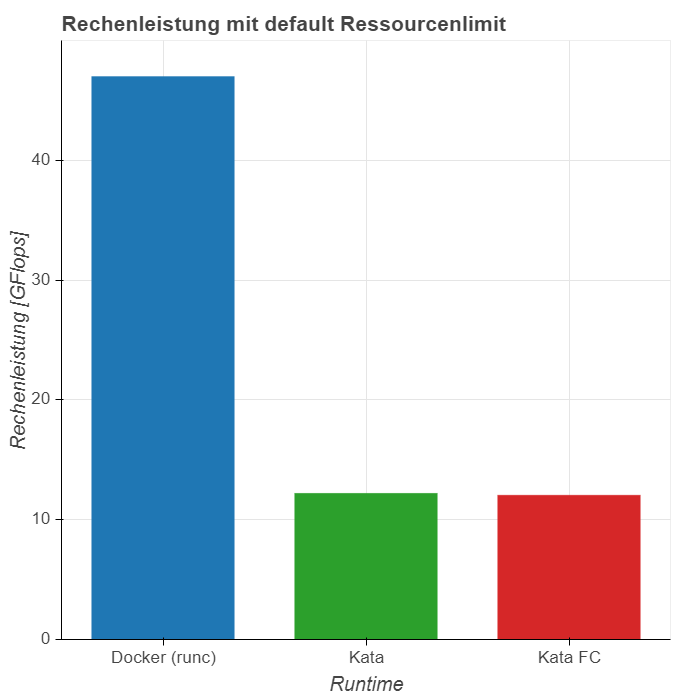
\includegraphics[width=.48\linewidth]{gfx/auswertung/linpack_default.png}} \quad
	\subfloat[Minimales Limit]
	{\label{fig:example-b}%
	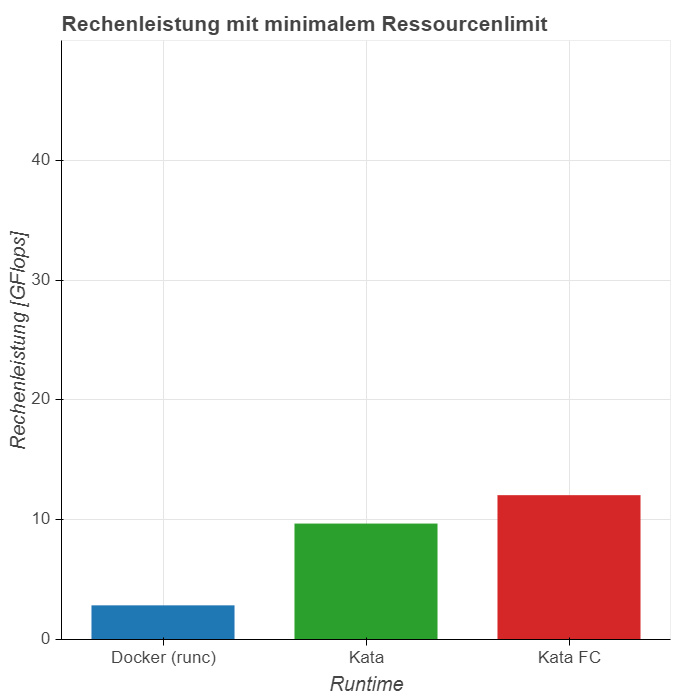
\includegraphics[width=.48\linewidth]{gfx/auswertung/linpack_min.png}} \\
	\subfloat[Maximales Limit]
	{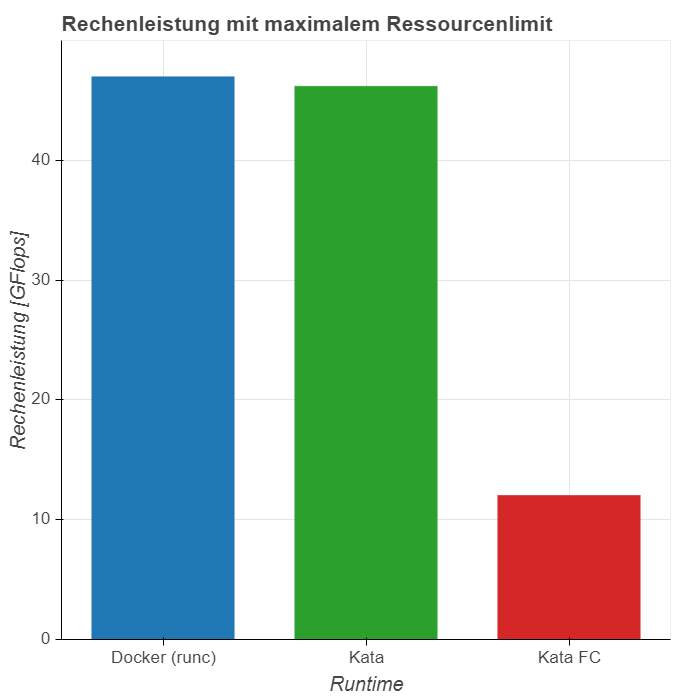
\includegraphics[width=.48\linewidth]{gfx/auswertung/linpack_max.png}} \quad
	\caption[Ergebnisse des Linpack Benchmarks]{Ergebnisse des Linpack Benchmarks nach Ressourcenlimits}
	\label{fig:linpackergebnisse}
\end{figure}

\newpage

\section{Einhaltung von Ressourcenlimits}
\label{sec:resslimits}
Die Untersuchungen zur Leistungsfähigkeit werden dazu verwendet um festzustellen, ob die gesetzten Ressourcenlimits Anwendung finden. Dieses Ergebnis wird für die Bewertung in Abschnitt \ref{sec:auswertung_dos} benötigt. Für die Runtimes Nabla und Kata FC ist nicht vollständig dokumentiert, inwieweit die Ressourcenlimits angewendet werden. 

Werden die Graphen zum Arbeitsspeicherverbrauch betrachtet, wird ersichtlich, dass Nabla bei jedem Ressourcenlimit den gleichen Verbrauch hat. Aus diesem Grund wird davon ausgegangen, dass Nabla keine Limitierung des Arbeitsspeichers vornimmt, vgl. Abbildung \ref{fig:ram_go} und \ref{fig:ram_python}. Bei der Untersuchung zur Webserverleistung unterscheidet sich die Leistung von Nabla bei den einzelnen Limits nicht. Nabla wendet hier keine Ressourcenlimitierung an.
In den Graphen zum Arbeitsspeicherverbrauch verläuft die Kurve von Kata FC mit maximalem Limit meist über der von default und minimalem Limit, vgl. Abbildung \ref{fig:ram_httpd}, \ref{fig:ram_nginx} und \ref{fig:ram_python}. Beim Betrieb des Images Go Httpd ist dieser Abstand kaum festzustellen, vgl. Abbildung \ref{fig:ram_go}. Die Limitierung des Arbeitsspeichers scheint also Auswirkungen auf den Verbrauch zu haben. Dabei ist anzunehmen, dass die Limitierung auf \ac{VM} Ebene und nicht für den Container in der \ac{VM} erfolgt. 

Zur Untersuchung der Rechenleistung mithilfe des Linpack Benchmarks werden die Ergebnisse dieses Benchmarks nicht gewichtet und in GFlops angegeben. Die Werte sind Tabelle \ref{tbl:linpackergebnisingflops} zu entnehmen. Dabei wird ersichtlich, dass sich die Ergebnisse von Kata FC bei den einzelnen Limits kaum unterscheiden. Bei den anderen Kandidaten Docker und Kata jedoch schon. Aus diesem Grund wird angenommen, dass Kata FC keine Limitierung der Prozessoren vornimmt.
Derzeit wendet Nabla keine Ressourcenlimitierung an und Kata FC nur im Bereich des Arbeitsspeichers.

\begin{table}[h]
	\myfloatalign
	\small 
	\begin{tabularx}{\textwidth}{Xrrr} \hline
		\spacedlowsmallcaps{Limit} & \spacedlowsmallcaps{Docker} & \spacedlowsmallcaps{Kata} & \spacedlowsmallcaps{Kata FC} \\ \hline
		default & 46,97 & 12,19 & 12,03 \\
		min & 2,81 & 9,64 & 12,02 \\
		max & 46,96 & 46,17 & 12,02 \\ \hline
		\textbf{Schnitt} & 32,25 & 22,67 & 12,02\\\hline
	\end{tabularx}
	\caption[Ergebnisse des Linpack Benchmarks in GFlops]{Ergebnisse des Linpack Benchmarks in GFlops}
	\label{tbl:linpackergebnisingflops}
\end{table}

\section{Sicherheit}
Für die Bewertung der Sicherheit werden in Abschnitt \ref{sec:sicherheit_kriterien} verschiedene Angriffsszenarien als Kriterien aufgestellt. Diese werden für die Kandidaten Docker, Kata, Kata FC und Nabla betrachtet. Die Bewertung erfolgt dabei qualitativ und wird im Bereich eins bis fünf vorgenommen. Die Bewertung durch die Skala ist der Tabelle \ref{tbl:skala_sec} zu entnehmen. In dieser Skala erhält Docker in jeder Bewertung eine drei. Dadurch ist gewährleistet, dass auch zukünftig andere Kandidaten mit Docker nach dieser Methode vergleichen werden können.

\begin{table}[h]
	\small 
	\myfloatalign
	\begin{tabularx}{\textwidth}{rX} \hline
		\spacedlowsmallcaps{Wert} & \spacedlowsmallcaps{Bedeutung} \\ \hline
		1 & Angriff ist deutlich wahrscheinlicher als bei Docker \\
		2 & Angriff ist wahrscheinlicher als bei Docker\\
		3 & Angriff ist so wahrscheinlich wie bei Docker \\
		4 & Angriff ist unwahrscheinlicher als bei Docker \\
		5 & Angriff ist deutlich unwahrscheinlicher als bei Docker \\\hline
	\end{tabularx}
	\caption[Skala für die Bewertung der Sicherheit]{Skala für die Bewertung der Sicherheit}
	\label{tbl:skala_sec}
\end{table}

\subsection{Ausbruch aus dem Container über Fehlkonfiguration}
Bei dieser Bedrohung werden zwei Kriterien abgeleitet. Zum einen, die Folgen einer fehlerhaften Nutzerkonfiguration bei einem kompromittierten Prozess im Container. Zum anderen, wie die Runtimes den Anwendungszugriff auf den Host Kernel standardmäßig restriktieren.

Der Angreifer, der einen Prozess in einem Container mit Docker übernimmt, kontrolliert einen Prozess, der auf dem Host System läuft. Dieser Prozess ist nur durch Namespaces, Control Groups und Capabilities von anderen Host Prozessen isoliert. Hat der Prozess root Rechte und der Container wird privilegiert ausgeführt, ist der Angreifer im Besitz eines root Prozesses auf dem Host und kann den Host übernehmen. Docker kann Systemaufrufe mit Seccomp filtern. Standardmäßig werden 44 der über 300 Aufrufe geblockt \cite[vgl.][]{DockerInc..20191203}.

Wird bei Kata ein Prozess im Container übernommen, muss der Angreifer den \ac{VM} Kernel und die Isolierung durch die \ac{VM} überwinden, um den Host zu kompromittieren. Der Angriff ist also durch die vielen Isolierungsschichten deutlich unwahrscheinlicher als bei Docker. Kata verwendet keine Filterung von Systemaufrufen. Dadurch war es in der Vergangenheit möglich Systemaufrufe zu verwenden, die es ermöglichten Fehler in der Dateisystemimplementierung des Hosts auszunutzen \cite[vgl.][]{TheMITRECorporation.2018}. Damit ist noch kein Ausbruch möglich, es zeigt aber, dass die Minimierung der Angriffsvektoren sinnvoll ist \cite[vgl.][]{Nablacontainers.20190515}. Grundsätzlich muss der Angreifer aber immer die Container-Virtualisierung und die \ac{VM} überwinden. Daher ist ein Containerausbruch unwahrscheinlicher als bei Docker. Diese Bewertung gilt genauso  für Kata FC, da die gleiche Architektur verwendet wird.

gVisor verwendet für den Containerbetrieb Sentry als Kernel im Userspace. Wird ein Programm im Container übernommen und die Isolierung des Containers überwunden, hat der Angreifer Zugriff auf Sentry und damit einen Prozess im Userspace. Der Angreifer müsste also die Rechte dieses Prozesses ausweiten, um den Host zu kompromittieren. Damit ist ein Angriff unwahrscheinlicher als bei Docker. gVisor verwendet Seccomp als Filter zwischen dem Container und Sentry und zwischen Sentry und dem Host Kernel \cite[vgl.][2]{EthanG.Young.2019}. Daher ist ein Containerausbruch deutlich unwahrscheinlicher als bei Docker.

Eine Anwendung in Nabla wird auf einem Unikernel ausgeführt. Eine kompromittiere Applikation ist daher nicht in der Lage einen anderen Prozess zu starten, da ein Unikernel nur einen Prozess ausführen kann \cite[vgl.][S. 109 f.]{UdoSeidel.2018}. Dadurch ist ein Ausbruch sehr unwahrscheinlich. Nabla verwendet eine sehr restriktive Seccompfilterung, zugelassen sind nur sieben verschiedene Aufrufe   \cite[vgl.][109]{UdoSeidel.2018}. Weiter wird derzeit kein Zugriff auf Volumes unterstützt \cite[vgl.][]{Nablacontainers.20190501}. Angriffe auf Dateisystemebene sind also nicht möglich. Aus diesen Gründen ist ein Containerausbruch sehr unwahrscheinlich.

\subsection{Ausbruch aus dem Container über einen Kernel Exploit}
Über einen Exploit im Linux Kernel ist es möglich, die Isolierung von Containervirtualisierung mit Docker zu überwinden \cite[vgl.][9]{OWASP.2019}. Im schlimmsten Fall erhält der Angreifer damit privilegierte Rechte auf dem Host.
Das Betriebssystem in den \acp{VM} von Kata ist Clear Linux  \cite[vgl.][107]{UdoSeidel.2018}. Auf dieses sind Linux Kernel Exploits grundsätzlich anwendbar. Danach müsste ein Angreifer noch die Virtualisierung überwinden. Dadurch ist der Angriff unwahrscheinlicher als bei Docker.
Bei Kata FC wird statt Clear Linux Firecracker verwendet. Dieses hat einen reduzierten Funktionsumfang und bietet damit einen kleineren Angriffsvektor als Clear Linux  \cite[vgl.][]{ArunGupta.2018}. Ein Containerausbruch ist damit deutlich unwahrscheinlicher als bei Docker.
Linux Kernel Exploits sind auf Container mit gVisor nicht anwendbar, da diese Sentry als Kernel verwenden. Wird über einen Exploit aus dem Container ausgebrochen, hat der Angreifer nur die Rechte vom Sentry Prozess und nicht die des Kernels. Eine Host Kompromittierung ist daher unwahrscheinlich.
Nabla verwendet den Unikernel anstelle des Linux Kernels. Die Entwicklung eines Exploits für diesen ist schwerer, da er nur Funktionen enthält, die für die Ausführung der Applikation benötigt werden. Wird der Unikernel übernommen, muss ein Angreifer noch Solo kompromittieren, um Zugriff auf den Host zu erlangen. Ein Ausbruch mit einem Kernel Exploit ist daher sehr unwahrscheinlich.

\subsection{Denial of Service Angriff}
\label{sec:auswertung_dos}
Runtimes können einen \ac{DoS} Angriff auf einen Container nur schwer verhindern. Durch das Setzen von Ressourcenlimits für einzelne Container ist es aber möglich, die anderen Dienste in Containern auf dem gleichen Host nicht auszubremsen. Die Bewertung wird für die Möglichkeiten der Limitierung von Prozessor und Arbeitsspeicher vorgenommen.
Für Docker können Limits für die Verwendung von Prozessor und Arbeitsspeicher gesetzt werden. Genauso kann die Ressourcennutzung mit Kata und gVisor eingeschränkt werden. Beide erhalten die gleiche Wertung wie Docker. Kata FC bietet keine Limitierung der Prozessorleistung. Ein DoS Angriff hat damit eine große Auswirkung. Kata FC wird bezüglich der Prozessorlimitierung mit eins bewertet. Die Arbeitsspeichernutzung lässt sich mit Kata FC einschränken, daher erhält es die gleiche Wertung wie Docker. Die Auswertung in Abschnitt \ref{sec:resslimits} hat gezeigt, dass Nabla keine Limitierung unterstützt. Daher wird die Runtime mit eins bewertet.

\subsection{Ergebnis}
Das Ergebnis der Untersuchung ist in Tabelle \ref{tbl:sec_ergebnisse} zusammengefasst. Dabei wird für die Bedrohungen der Durchschnitt der einzelnen Kriterien gebildet. Diese Werte werden in der Bewertung für eine Empfehlung verwendet.

\begin{table}[ht]
	\myfloatalign
	\small 
	\begin{tabularx}{\textwidth}{Xrrrrr} \hline
		\spacedlowsmallcaps{Kriterium} & \spacedlowsmallcaps{Docker} & \spacedlowsmallcaps{Kata} & \spacedlowsmallcaps{Kata FC} &  \spacedlowsmallcaps{gVisor} & \spacedlowsmallcaps{Nabla} \\ \hline
		Fehlerhafte Nutzerkonfig. & 3 & 5 & 5 & 4 & 5 \\
		Filterung der Kernelzugriffe & 3 & 4 & 4 & 5 & 5 \\ \hline
		\textbf{Schnitt Fehlkonfiguration} & 3 & 4,5 & 4,5 & 4,5 & 5 \\ \hline
		\textbf{Kernel Exploit} & 3 & 4 & 5 & 4 & 5 \\ \hline
		Prozessor & 3 & 3 & 1 & 3 & 1 \\
		Arbeitsspeicher & 3 & 3 & 3 & 3 & 1 \\ \hline
		\textbf{Schnitt DoS Angriff} & 3 & 3 & 2 & 3 & 1 \\ \hline
	\end{tabularx}
	\caption[Ergebnisse der Sicherheitsbewertung]{Ergebnisse der Sicherheitsbewertung,}
	\footnotesize Skala: 1 (Angriff sehr wahrscheinlich) bis 5 (Angriff sehr unwahrscheinlich)
	\label{tbl:sec_ergebnisse}
\end{table}

\section{Benutzbarkeit}
Die Kriterien für die Bewertung der Benutzbarkeit werden in Abschnitt \ref{sec:benutzbarkeit_krit} beschrieben. Diese werden für die Kandidaten Docker, Kata, Kata FC und Nabla betrachtet. Die Bewertung erfolgt dabei qualitativ und wird im Zahlenbereich eins bis fünf vorgenommen. Dabei wird mit einer Eins deutlich schlechter und einer Fünf deutlich besser als Docker bewertet. In dieser Skala erhält Docker in jeder Bewertung eine drei. Dadurch ist sichergestellt, dass auch zukünftig andere Kandidaten mit Docker nach dieser Methode verglichen werden können.

Alle Kandidaten lassen sich in Docker und Kubernetes integrieren. Dabei können auch alle Runtimes parallel in Docker auf einem System verwendet werden. Dazu müssen die Runtimes in der \lstinline[]|daemon.json| konfiguriert und beim Start eines Containers mit \lstinline[]|--runtime| festgelegt werden \cite[vgl.][]{UdoSeidel.2018}. Für Kata FC muss zusätzlich der Speichertreiber konfiguriert werden. Daher wird Kata FC mit zwei und die anderen Kandidaten mit drei bewertet. 

Für Kubernetes kann Kata, Kata FC, gVisor und Nabla als Plugin von containerd verwendet werden. Ein Pod, der mit der "`Annotation"' \lstinline[]|io.kubernetes.cri.untrusted-workload: "true"| gestartet wird, wird dann mit der konfigurierten Runtime und nicht runc betrieben \cite[vgl.][]{katacontainers.20190613, gVisor.20191024, nablacontainers.20181105}. Für die Verwendung von Nabla müssen aber noch einige Netzwerkkonfigurationen angepasst werden  \cite[vgl.][]{nablacontainers.20181105}. Daher wird Nabla für die Integration in Kubernetes mit zwei, alle Anderen mit drei bewertet.

Alle Kandidaten außer Nabla liefern Binärdateien auf ihren Webseiten oder stellen Pakete für die meisten Linux Systeme bereit. Für die Installation von Nabla muss der Quellcode selbst übersetzt werden \cite[vgl.][]{UdoSeidel.2018}. Aus diesem Grund wird Nabla für die Installation mit zwei, alle anderen mit drei bewertet.
Die Systemvoraussetzungen sind in vielen Teilen ähnlich, alle sind für Linux Systeme konzipiert. Kata und Kata FC setzten für die Installation aber ein System mit Hardwarebeschleunigung voraus  \cite[vgl.][108]{UdoSeidel.2018}. Daher können diese beiden Kandidaten nicht in virtuellen Maschinen ohne geschachtelte Virtualisierung verwendet werden. Die Kandidaten gVisor und Nabla erhalten in diesem Kriterium drei und Kata und Kata FC einen Punkt. 

Die Runtimes Kata, Kata FC und gVisor sind grundsätzlich mit Docker Images kompatibel. Für Nabla müssen eigene Images erstellt werden. Daher wird Nabla hier mit eins und die anderen Kandidaten mit drei bewertet. Während den Messungen sind bei allen Kandidaten, außer Kata, Probleme aufgetreten: Kata FC stürzt regelmäßig beim Beenden von Containern mit dem Tomcat Image ab. Der Betrieb von Httpd Container ist mit gVisor nicht möglich, da diese des Öfteren abstürzt. Weiter kann der Linpack Benchmark auf gVisor nicht gestartet werden, da einer der benötigen Systemaufrufe nicht unterstützt wird. Nabla stürzt beim Betrieb des Node Express Images regelmäßig ab und eine Skalierung von Python Tornado ist über elf Container nicht möglich. Aus den genannten Gründen, erhält Kata in diesem Kriterium drei, Kata FC zwei und gVisor und Nabla einen Punkt.

Da sich alle Kandidaten mit Docker verwenden lassen, sollten sie auch die Befehle, die sonst von runc ausgewertet und umgesetzt werden, auch anwenden. Kata unterstützt bisher die Befehle \lstinline[]|checkpoint| und \lstinline[]|restore| nicht \cite[vgl.][]{KataContainers.20190919}. Kata FC unterstützt die bei Kata genannten Befehle auch nicht. Weiter wendet Kata FC keine Ressourcenlimits an und die Unterstützung von Container Volumes und Speicher Typen, neben Block Speichern, fehlen bisher \cite[vgl.][]{katacontainers.20190123}. Nabla unterstützt derzeit keine  Container Volumes, Ressourcenlimits oder das Schreiben von Dateien außerhalb von /tmp unterstützt \cite[vgl.][]{nablacontainers.20190402}. Für gVisor sind keine Probleme bekannt, daher wird diese Runtime mit drei Bewertet. Kata erhält zwei und Kata FC und Nabla einen Punkt.

Die Zusammenfassung der Bewertung ist Tabelle \ref{tbl:benutzbarkeit_ergebnis} zu entnehmen. 


\begin{table}[hb]
	\myfloatalign
	\small
	\begin{tabularx}{\textwidth}{Xrrrrr} \hline
		\spacedlowsmallcaps{Kriterium} & \spacedlowsmallcaps{Docker} & \spacedlowsmallcaps{Kata} & \spacedlowsmallcaps{Kata FC} &  \spacedlowsmallcaps{gVisor} & \spacedlowsmallcaps{Nabla} \\ \hline
		Integration in Docker                                        & 3      & 3    & 2       & 3      & 3     \\
		Integration in Kubernetes                                    & 3      & 3    & 3       & 3      & 2     \\
		Installation                                                 & 3      & 3    & 3       & 3      & 2     \\
		Systemvoraussetzungen                                        & 3      & 1    & 1       & 3      & 3     \\
		Image Kompatibilität                                  & 3      & 3    & 3       & 3      & 1     \\
		Probleme mit Images                    & 3      & 3    & 2       & 1      & 1     \\
		Docker Funktionen                         & 3      & 2    & 1       & 3      & 1     \\ \hline
	\end{tabularx}
	\caption[Ergebnisse der Benutzbarkeitsbewertung]{Ergebnisse der Benutzbarkeitsbewertung,}
	\footnotesize Skala: 1 bis 5, größer ist besser
	\label{tbl:benutzbarkeit_ergebnis}
\end{table}

\section{Bewertung}
\label{sec:bewertung}
Für die Bewertung wird die Methode der Entscheidungsanalyse von Dittmer weitergeführt. Dazu werden die Gewichtungen aus \ref{sec:zielgewichtung} verwendet. Es wird ein relativer Vergleich der Kandidaten durchgeführt. Dazu erhält die Alternative mit der höchsten Bewertung (Zielertrag) in einer Kategorie die höchste Punktzahl, in diesem Fall zehn Punkte. Diese Punktzahl wird Zielwert genannt. Die Alternative mit der geringsten Bewertung (Zielertrag) erhält nur einen Punkt. Bei den dazwischenliegenden Bewertungen wird der Zielwert linear zwischen eins und zehn interpoliert. Jeder einzelne Zielwert wird mit dem Gewicht des Kriteriums multipliziert. Dieses Ergebnis wird als Teilnutzen bezeichnet. Durch die Bildung der Summe aller Teilnutzen pro Kandidaten wird die Rangfolge der Kandidaten untereinander deutlich.  \cite[vgl.][S. 151 ff.]{Dittmer.2002}

Das Ergebnis ist der Tabelle \ref{tbl:bewertung} zu entnehmen. Diese Methode wird einzeln für die drei Bereiche Leistungsfähigkeit, Sicherheit und Benutzbarkeit durchgeführt. Die Gewichtung der Bereiche erfolgt wie in \ref{sec:zielgewichtung} beschrieben. In der Zeile Gesamt werden die Ergebnisse der Bereiche im Verhältnis 2:2:1 zusammengefasst. Da jeder Bereich durch die prozentuale Gewichtung die gleiche Anzahl an Punkten maximal vergeben kann, ist eine solche Zusammenfassung möglich.

Nach dieser Methode erhalten wir die Rangfolge der Alternativen zu Docker. Kata ist mit 3880,53 Punkten die beste Alternative, danach folgen Kata FC mit 3538,79, Nabla mit 3479,16 und gVisor mit 3036,45 Punkten. Nach dieser Bewertung schneidet Docker mit 2898,24 am schlechtesten ab.

\newcommand{\STAB}[1]{\begin{tabular}{@{}c@{}}#1\end{tabular}}
\begin{sidewaystable}
	\footnotesize
	\setlength{\tabcolsep}{0.8mm} % Spaltenabstand anpassen
	\centering
\begin{tabular}{|l|l|l|rrr|rrr|rrr|rrr|rrr|} \hline
	& & & \multicolumn{3}{c|}{\spacedlowsmallcaps{Docker}} & \multicolumn{3}{c|}{\spacedlowsmallcaps{Kata}} & \multicolumn{3}{c|}{\spacedlowsmallcaps{Kata FC}} & \multicolumn{3}{c|}{\spacedlowsmallcaps{gVisor}} & \multicolumn{3}{c|}{\spacedlowsmallcaps{Nabla}} \\
	& \spacedlowsmallcaps{Kriterum} & \spacedlowsmallcaps{Gewichtung} & {\tiny Zielertrag} & {\tiny Zielwert} & {\tiny Teilnutzen} & {\tiny Zielertrag} & {\tiny Zielwert} & {\tiny Teilnutzen} & {\tiny Zielertrag} & {\tiny Zielwert} & {\tiny Teilnutzen} & {\tiny Zielertrag} & {\tiny Zielwert} & {\tiny Teilnutzen} & {\tiny Zielertrag} & {\tiny Zielwert} & {\tiny Teilnutzen} \\ \hline
	\multirow{7}{*}{\STAB{\rotatebox[origin=c]{90}{Leistungsfähigkeit}}} & Webserverleistung & 28,57 & 100,00 & 8,11 & 231,73 & 109,87 & 9,19 & 262,54 & 60,83 & 3,83 & 109,41 & 34,94 & 1,00 & 28,57 & 117,29 & 10,00 & 285,71 \\
	& Arbeitsspeichernutzung & 9,52 & 100,00 & 8,13 & 77,44 & 197,10 & 1,00 & 9,52 & 103,67 & 7,86 & 74,88 & 117,34 & 6,86 & 65,31 & 74,56 & 10,00 & 95,24 \\
	& Dauer des Startens & 14,29 & 100,00 & 10,00 & 142,86 & 183,02 & 6,55 & 93,51 & 316,31 & 1,00 & 14,29 & 104,99 & 9,79 & 139,89 & 234,70 & 4,40 & 62,79 \\
	& Dauer des Entfernens & 4,76 & 100,00 & 6,89 & 32,81 & 140,55 & 3,56 & 16,95 & 171,71 & 1,00 & 4,76 & 104,94 & 6,48 & 30,88 & 62,14 & 10,00 & 47,62 \\
	& Netzwerkbandbreite & 19,05 & 100,00 & 10,00 & 190,48 & 99,92 & 9,97 & 189,82 & 99,56 & 9,81 & 186,89 & 78,98 & 1,00 & 19,05 & 89,49 & 5,50 & 104,76 \\
	& Prozessorleistung & 23,81 & 100,00 & 1,00 & 23,81 & 155,78 & 9,41 & 224,16 & 159,66 & 10,00 & 238,10 & 129,83 & 5,50 & 130,95 & 129,83 & 5,50 & 130,95 \\ \cline{2-18} 
	& \textbf{Summe Leistungsfähigkeit} & & & & 699,12 & & & 796,51 & & & 628,32 & & & 414,66 & & & 727,08 \\ \hline
	\multirow{4}{*}{\STAB{\rotatebox[origin=c]{90}{Sicherheit}}}& Ausbruch über Fehlkonfig. & 33,33 & 3,00 & 1,00 & 33,33 & 4,50 & 7,75 & 258,33 & 4,50 & 7,75 & 258,33 & 4,50 & 7,75 & 258,33 & 5,00 & 10,00 & 333,33 \\
	& Ausbruch mit Kernel Exploit & 50,00 & 3,00 & 1,00 & 50,00 & 4,00 & 5,50 & 275,00 & 5,00 & 10,00 & 500,00 & 4,00 & 5,50 & 275,00 & 5,00 & 10,00 & 500,00 \\
	& Denial of Service Angriff & 16,67 & 3,00 & 10,00 & 166,67 & 3,00 & 10,00 & 166,67 & 2,00 & 5,50 & 91,67 & 3,00 & 10,00 & 166,67 & 1,00 & 1,00 & 16,67 \\ \cline{2-18} 
	& \textbf{Summe Sicherheit} & & & & 250,00 & & & 700,00 & & & 850,00 & & & 700,00 & & & 850,00 \\ \hline
	\multirow{8}{*}{\STAB{\rotatebox[origin=c]{90}{Benutzbarkeit}}}& Integration in Docker & 17,86 & 3,00 & 10,00 & 178,57 & 3,00 & 10,00 & 178,57 & 2,00 & 1,00 & 17,86 & 3,00 & 10,00 & 178,57 & 3,00 & 10,00 & 178,57 \\
	& Integration in Kubernetes & 14,29 & 3,00 & 10,00 & 142,86 & 3,00 & 10,00 & 142,86 & 3,00 & 10,00 & 142,86 & 3,00 & 10,00 & 142,86 & 2,00 & 1,00 & 14,29 \\
	& Installation & 3,57 & 3,00 & 10,00 & 35,71 & 3,00 & 10,00 & 35,71 & 3,00 & 10,00 & 35,71 & 3,00 & 10,00 & 35,71 & 2,00 & 1,00 & 3,57 \\
	& Systemvoraussetzungen & 7,14 & 3,00 & 10,00 & 71,43 & 1,00 & 1,00 & 7,14 & 1,00 & 1,00 & 7,14 & 3,00 & 10,00 & 71,43 & 3,00 & 10,00 & 71,43 \\
	& Image Kompatibilität & 25,00 & 3,00 & 10,00 & 250,00 & 3,00 & 10,00 & 250,00 & 3,00 & 10,00 & 250,00 & 3,00 & 10,00 & 250,00 & 1,00 & 1,00 & 25,00 \\
	& Probleme mit Images & 21,43 & 3,00 & 10,00 & 214,29 & 3,00 & 10,00 & 214,29 & 2,00 & 5,50 & 117,86 & 1,00 & 1,00 & 21,43 & 1,00 & 1,00 & 21,43 \\
	& Docker Funktionen & 10,71 & 3,00 & 10,00 & 107,14 & 2,00 & 5,50 & 58,93 & 1,00 & 1,00 & 10,71 & 3,00 & 10,00 & 107,14 & 1,00 & 1,00 & 10,71 \\ \cline{2-18} 
	& \textbf{Summe Benutzbarkeit} & & & & 1000,00 & & & 887,50 & & & 582,14 & & & 807,14 & & & 325,00 \\ \hline
	&\textbf{Gesamt} &  & & & 2898,24 & & & 3880,53 & & & 3538,79 & & & 3036,45 & & & 3479,16  \\ \hline
\end{tabular}
	\caption{Bewertung der Kandidaten}
	\label{tbl:bewertung}
\end{sidewaystable}